\documentclass[12pt]{article}
\usepackage[english]{babel}
\usepackage[utf8]{inputenc}
\usepackage{amsmath}
\usepackage{amssymb}
\usepackage{amsthm}
\usepackage{hyperref}
\usepackage{graphicx}
\usepackage{subcaption}
\usepackage{xcolor}
\usepackage{algorithm}
\usepackage{algpseudocode}
\usepackage{parskip}

\graphicspath{{figures/}}

\newcommand{\todo}[1]{\textcolor{red}{#1}}



\newtheorem{thm}{Theorem}
\newtheorem{proposition}{Proposition}
\newtheorem{lemma}{Lemma}
\newtheorem{example}{Example}

\theoremstyle{definition}
\newtheorem{definition}{Definition}[section]


\title{\Large Distributed Trajectories under Mobile Phone Network: \\Empirical Estimation on Origin-Destination Matrix and Time-inhomogeneous Simulation}

\author{Liyuan Zhang\\[2cm]{\large Department of Mathematics}\\[0.2cm]{\large Uppsala University}\\[2cm]{\large Supervisor: Raazesh Sainudiin}}

\hypersetup{
    colorlinks=true,
    linkcolor=black,
    urlcolor=cyan,
    citecolor=red,
    filecolor=green
}




\begin{document}

\maketitle\newpage


\tableofcontents\newpage




\begin{abstract}
  A trajectory is the movement of an object in space as time goes by, aka ‘spatiotemporal’. Aside from all the properties an ordinary trajectory possesses, the primary characteristic of a distributed trajectory is the uncertainty of its positioning. Each movement will generate a (probability) distribution so that the location for each record is not deterministic. This thesis will present the dynamics of distributed trajectories under Mobile Phone Network (MPN) of certain areas in Sweden, by demonstrating a series of visualisations and how they are applied in the real world with estimation and simulation of certain spatiotemporal Markov models. Our main objective is to develop and test estimation and simulation algorithms that can scale to arbitrarily large MPN datasets.
\end{abstract}

\section{Introduction}
\subsection{Background}
Mobile technology has been making huge impacts on humans and society, which only became more evident after the emergence of smartphones and the popularity of big data technologies. Every day, while people use various smartphone applications, a huge amount of data is generated and analyzed in order to provide exclusive services for each user. Among all of the applications, the location-accessed setting is very common and, in most cases, default. For example, for a simple Weather app, we cannot possibly know the weather accurately to the region where we are currently locating if we do not enable the location service. The fact that other examples such as Uber, Google Maps, Yelp, and Foodora (a platform that offers food delivery for restaurants in Nordics) are all location-based is self-explanatory. This technological integration of mobile and spatiotemporal elements has undoubtedly produced a long-lasting effect on today’s society -- from providing conveniences for people’s life to helping visionaries make blueprints for smart cities. 

All those applications we listed above hinge on precise positioning. Imagine the potential consequences if Google Maps makes positioning errors while driving. In the field of human mobility study, mobile phone data has always been a great resource based on the intuitively plausible assumption that the device/individual’s positioning corresponds to the cell tower which processes its Mobile Phone Network (MPN) or Call Details Record (CDR). This is the main conception of Voronoi-based positioning. Recently, certain studies have demonstrated that this measure of positioning is not as precise as it is assumed to be. A considerable discrepancy is revealed by comparing volunteers’ MPN and GPS records between the mobile device and the cell tower that served the device \cite{closest_antenna_fallacy_2021}. A certain probabilistic approach has been investigated to achieve more precise device positioning due to the low credibility of Voronoi-based positioning \cite{prob_posit_mpn_2021}. This study reveals the fallacy of traditional Voronoi-based positioning and motivates the origins for distributed trajectories.

\subsection{Introduction to Mobile Data}
\label{sec:mobile_data}
Aside from those enterprises we mentioned above who own their proprietaries, the amplest mobile data resources are usually from mobile network operators themselves in their local countries. For example, the most widely known mobile telecommunication companies in the US are AT\&T and T-Mobile; in Sweden, there are Telia, Tele2, Telenor, etc. 

One type of location-based mobile data is called Call Details Record (CDR), produced by carriers when telecommunication transactions (voice call or text message) occur. For CDR data, besides basic information such as clients’ IDs (which are confidential) and call types, attributes such as call time, duration, and geographical coordinates (latitude and longitude) of devices are more useful for mobility study. This is the general form of aggregated CDR data. However, for non-aggregated CDR, instead of the whole duration of that phone call, it consists of a series of statuses. For each status in each timestamp, even during the same call, the cell tower that served that device may change \cite{prob_posit_mpn_2021}.

Another type of location-based mobile data (the data used in this thesis), is called Mobile Phone Network (MPN), or Cellular Network. It is in some ways similar to non-aggregated CDR as it is recorded and documented in every timestamp by potentially different cell towers as long as the 'Mobile Data' setting is turned on. This makes MPN data more thorough, understandable, and even live-streamable. A sample of MPN data is shown in Figure \ref{fig:mpn_sample}, where a pair of \(X_{i}\) and \(Y_{i}\) could also be represented as a cell tower, or a polygon. We will elaborate on this in the following sections. 

\begin{figure}
  \centering
  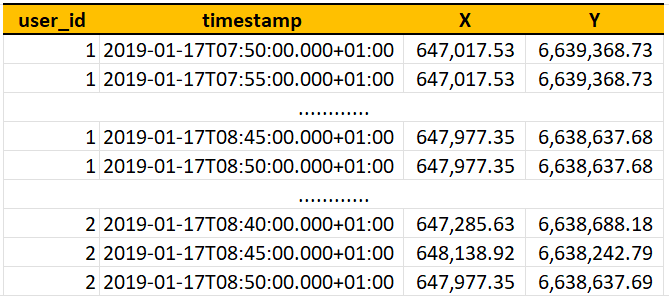
\includegraphics[width=12cm]{mpn_sample.jpg}
  \caption{Sample of MPN data}
  \label{fig:mpn_sample}
\end{figure}

On top of this, the idea of distributed trajectories originated from the fact that the uncertainty of positioning by cell towers, which means the trajectory records, as Figure \ref{fig:mpn_sample} reveals, are not meant to be \(100\%\) accurate. Each trajectory with a deterministic but imprecise location, will be reformulated according to this uncertainty. Thus turning into a trajectory with probabilistic locations, also known as, distributed trajectory.

\subsection{Goals of this Thesis}
This thesis will present the whole dynamics of distributed trajectories under Mobile Phone Network (MPN) of certain areas in Sweden (approximately from Uppsala to Stockholm). We start by utilizing a sample of Mobile Phone Network (MPN) data to generate distributed trajectories and observing how it evolves as certain parameters change; we study its mobility patterns by constructing certain forms of visualization such as Origin-Destination matrix and Transition matrix, and we simulate distributed trajectories given certain states and models to forecast future patterns. Exploring scalable algorithms for big MPN data is also one of our main goals. The code for this thesis can be found at: \url{https://github.com/lizh7573/distributed_trajectories_mpn}. \newpage



%=========================================================%



\section{Markov chain in Trajectory Analysis}
In this section, we will be focusing on some important concepts of a Markov chain that will be used in this thesis. We will not cover all of the aspects in this field, but only some fundamental concepts and how they are related to the mobility/trajectory area we are studying. Then the formal definition of trajectory and an example will be given.

\begin{definition}[\textbf{Markov chain}]
  \label{def:markov_chain}
  A Markov chain is a stochastic process modeling a sequence of states \((X_{t})_{t \geq 0}\), where the probability of the next state only depends on the current state, which could be expressed as:\\
  \begin{equation*} 
  P(X_{t}|X_{1},X_{2},...,X_{t-1}) = P(X_{t}|X_{t-1}) 
  \end{equation*}
\end{definition}

The property that the probability of the next state only depending on the current state is the Markov \(memorylessness\) property of a Markov chain. However, precisely speaking, it is hard to ignore all the historical records in mobility/trajectory study since objects usually mobilize with purpose. For example, the probability of moving backward is far less than moving forward for a reasonable trajectory; and it is almost impossible to jump to other regions all of sudden. Hence, we also introduce high-order Markov chain so that we can choose how many steps in the past could determine the probability of the next step.

\begin{definition}[\textbf{High-order Markov chain}]
  \label{def:markov_chain}
  A high-order Markov chain can be formulated to satisfy the following property:\\
  \begin{equation*} 
  P(X_{t}|X_{1},...,X_{t-N},...,X_{t-1}) = P(X_{t}|X_{t-N},...,X_{t-1}), t>N>0,
  \end{equation*} where the probability of the next state depends on the previous \(N\) states.
\end{definition}

\begin{definition}[\textbf{State space}]
  \label{def:state_space}
  The state space of a Markov chain is all possible values of \(X_i\) that compose a set \(\mathbb{S}\). \(\mathbb{S}\) can be either countable or uncountable.
\end{definition}

When it comes to mobility/trajectory study, space and time are the two most important elements to be considered. In our case, for a random variable \(X_i\), its realization \(x_i\) represents the geographical location at the time \(i\). We denote \(x_i\) = \(d\) as a data point, and the set of all data points is denoted as \(\mathbb{D}\) \cite{privacy_traj_co-traj_2019}. A sequence of \(d\) with chronological progress is what makes a trajectory. 

According to the sample data (Figure \ref{fig:mpn_sample}), each pair of \(X_i\) and \(Y_i\) could be represented as a cell tower or a polygon (we will cover this in the next section), which makes the state space countable. Plus, each record has been recorded at 5-min resolution, i.e., \(|i+1|-|i| = 5\). Therefore, the Markov chain in our case is categorized as discrete time and countable space Markov chain. Next we define a trajectory and the transition matrix.

\begin{definition}[\textbf{Trajectory}]
  \label{def:traj}
  A trajectory, denoted as \(r\), where \(r \subset \mathbb{D}\), is given by a sequence of data points \(d\), where \(d \in \mathbb{S} \times \mathbb{R_{+}}\). Given a finite interval of time, each data point is time non-overlapped, and the number of data points is finite \cite{privacy_traj_co-traj_2019}.
\end{definition}

\begin{definition}[\textbf{Transition matrix}]
  A transition matrix, also called a stochastic matrix, denoted as \textbf{P}, is a square matrix whose element in the \(m^{th}\) row and \(n^{th}\) column, \(p_{m,n}\), represents the probability of moving from \(m\) to \(n\). A transition matrix is row-normalised, that is:
  \[ \sum_{n=1}^{\left| \mathbb{S} \right|} p_{m,n} = 1, \left| \mathbb{S} \right|:= \textnormal{size of}\; \mathbb{S} \]
\end{definition} 

To sum up, let’s make a simple example. 

Below is a trajectory, \(r_1\), recorded by a volunteer's GPS device in Uppsala (see Figure \ref{fig:rand_traj_uppsala}). There are 15 data points in this trajectory, and each data point represents a location (state) that has been recorded only once at that time. From \(r_1\), if we are confident that the probabilities from \(d_1\) to \(d_2\), \(d_2\) to \(d_3\), ..., \(d_{14}\) to \(d_{15}\) are all \(100\%\), then a \(15 \times 15\) transition matrix \textbf{P} is formed with \(p_{m,m+1}=1\). We can take this simple example as a mock-up for our trajectory and distributed trajectory analysis.

\newpage

\begin{figure}
  \centering
  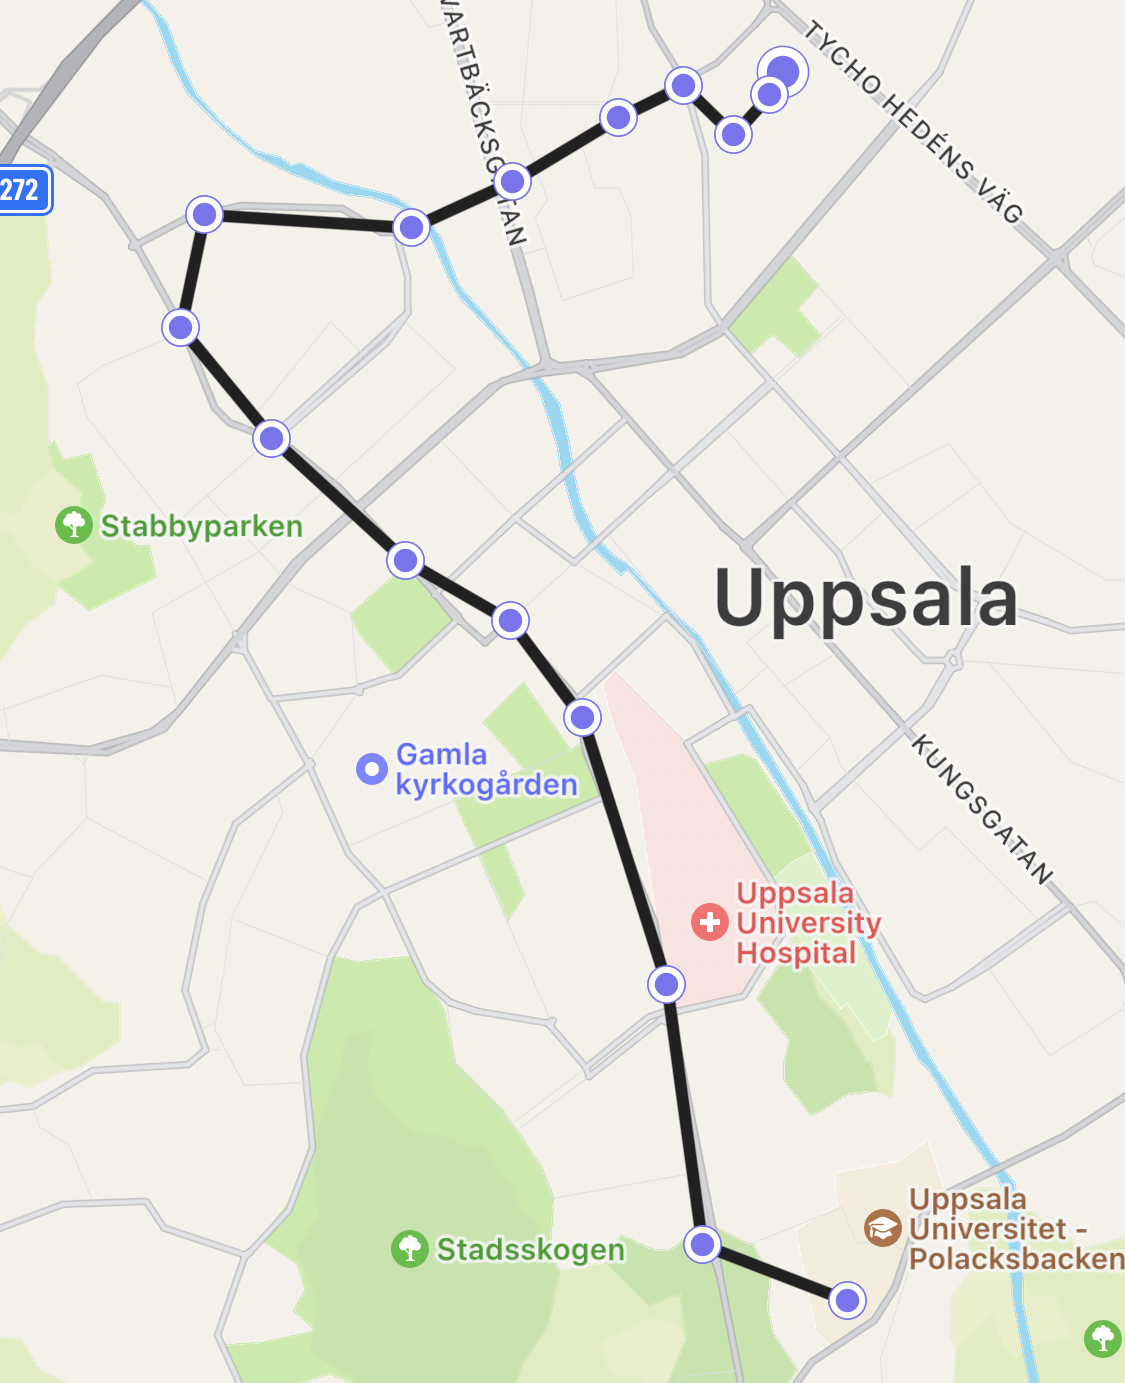
\includegraphics[width=6cm]{rand_traj_uppsala.jpg}
  \caption{Example of a trajectory, recorded by volunteer's GPS device}
  \label{fig:rand_traj_uppsala}
\end{figure}

Realistically, according to the research team from the Social and Economic Geography Department at Uppsala University and the Geography and Human Environment Department at Tel Aviv University, one cannot simply assume our mobile network is connected to the closest antenna when dealing with MPN data, and therefore the real locations do not always correspond to their pin records \cite{closest_antenna_fallacy_2021}. This brings us to distributed trajectories. \newpage




%=========================================================%




\section{Trajectories and Distributed Trajectories: Deterministic versus Probabilistic}
In this section, we first introduce the ideas behind distributed trajectories, to see under which circumstances distributed trajectories could exist, and how they could be generated from ordinary trajectories. Then we will introduce some concepts in the traditional Voronoi-based positioning, show how the whole mobile phone network is constructed, present trajectories under this framework in order to have a visualized intuition, and explain the fallacy of this approach. Finally, we will begin to generate distributed trajectories by using some empirical statistics, with both Voronoi polygons and rings of such polygons.

\subsection{Ideas behind Distributed Trajectories: Grid Partition with Gaussian Noise}
In the last example, we mentioned that only if we are 100\% confident that each transition was exactly the same location as the record displayed as we look back to the trajectory, can we have that transition matrix \textbf{P}, with:\\
\begin{equation*} 
p_{m,m+1}=1, m \in \mathbb{S}
\end{equation*} 

However, one can generally not guarantee such accuracy of each record with 100\% confidence. In order to fully comprehend the idea of distributed trajectories, we partition the map into numerous extremely fine grids. Formally, in the limit:\\
\[ \lim_{\lvert d \rvert \to 0} {\left|\mathbb{S}\right|}=\infty,  \]
where \(|d|\) is the distance between two data points (states).

With the map partitioned into even finer grids, the number of states in state space \(\mathbb{S}\) tends to infinity, which represents higher resolution, thus causing more frequent deviation. Since no matter how small the movement of objects, it could be seen as a transition, making positioning records even harder to be accurate. Therefore, we need to take probability into account. In this case, we consider adding Gaussian noise on arbitrarily fine but finite grids with \(\left|\mathbb{S}\right|<\infty.\)

\begin{definition}[\textbf{Gaussian noise}]
  \label{def:gaussian_noise}
  Gaussian noise is statistical noise of the Gaussian random variable. The probability density function \(f\) of a Gaussian random variable \(Z\) is given by:
  \begin{equation*}
  f(z)= \frac{1}{\sigma\sqrt{2\pi}} \exp^{-(z-\mu)^2/2\sigma^2}
  \end{equation*}
  where \(z\) represents the realized value of a random variable, \(\mu\) is mean and \(\sigma\) is standard deviation.
\end{definition}


In our case, the deviation from the location recorded can be seen as the noise, and we assume these noises are Gaussian-distributed. Algorithm \ref{alg:gauss-noise} gives our procedure for adding Gaussian noise to our data.

\begin{figure}
  \centering
  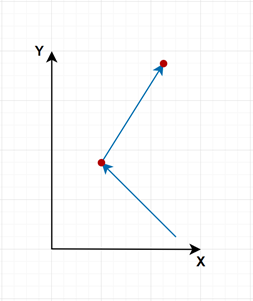
\includegraphics[width=5.5cm]{gaussian_noise_1}
  \captionsetup{justification=centering}
  \caption{Generate a random deterministic trajectory}
  \label{fig:gaussian_noise_1}
\end{figure}

The geographical information is given as \(X_{i}\) and \(Y_{i}\). The map is partitioned into a regular gird. Consider Figure \ref{fig:gaussian_noise_1} as our example, where axes \(x\) and \(y\) represent geographical coordinates. Each intersection of the regular grids lines can be seen as a state \(s\). The arrow represents both directional and chronological progress, and each red dot is a data point \(d\) recorded with information on both location and time. 

\begin{figure}
  \centering
  \begin{subfigure}[t]{0.4\textwidth}
    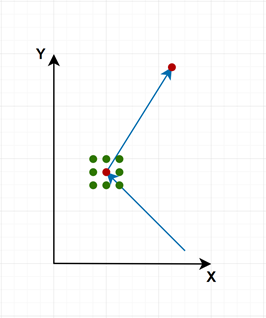
\includegraphics[width=\textwidth]{gaussian_noise_2.jpg}
    \caption{}
  \end{subfigure}
  \begin{subfigure}[t]{0.4\textwidth}
    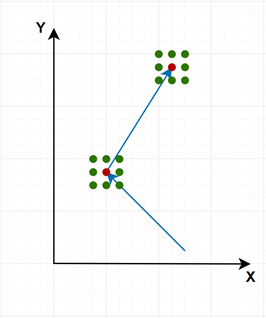
\includegraphics[width=\textwidth]{gaussian_noise_3.jpg}
    \caption{}
  \end{subfigure}
  
  \begin{subfigure}[t]{0.6\textwidth}
    \centering
    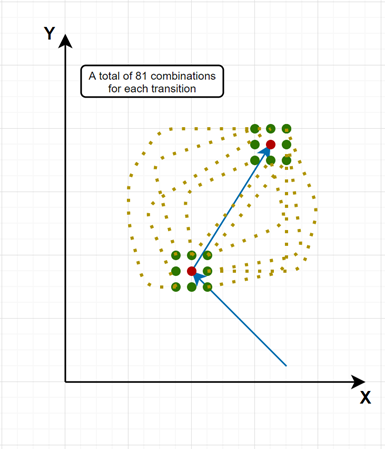
\includegraphics[width=\textwidth]{gaussian_noise_4.jpg}
    \caption{}
  \end{subfigure}
  \caption{Generate distributed trajectories under Grid partition by adding Gaussian noise}
  \label{fig:gaussian_noise}
\end{figure}

By adding Gaussian noise, each movement recorded would have a probability (in this case, Gaussian) distribution. This entire process is described and depicted in Figure \ref{fig:gaussian_noise}. 


\begin{algorithm}
  \caption{Algorithm for adding Gaussian noise on trajectories under Grid partition}
  \label{alg:gauss-noise}
  \begin{algorithmic}
    \Procedure{Gaussian}{$(x^{(t)},y^{(t)}),w,\mu,\sigma$}
    \Comment{parameters: current coordinate, width of distributed range, mean, standard deviation}
    \State \textbf{Enumeration} \((x^{(t)},y^{(t)})_{i=1,2,...,(2w+1)^2}\) \Comment{within width \(w\)}
    \For{\((x^{(t)},y^{(t)})_{i} \in Enumeration, i \in {1,2,...,(2w+1)^2}\)}
    \State \(p_{i} \gets Gaussian((x^{(t)}, y^{(t)})_{i}, w, \mu, \sigma)\)
    \EndFor
    \State \textbf{return} \(\{(x^{(t)}, y^{(t)})_{i}, p_{i}\}\)
    \EndProcedure
  \end{algorithmic}
\end{algorithm}

As we mentioned above, each red dot represents a record stored as an MPN observation, while each green dot can be seen as a probabilistic record on top of it. We take coordinates of each red dot, width of distributed range, and fixed mean and standard deviation as our inputs. Noted, we define the width as 1 in this case. With width \(w\) equals to 1, there will be \((2w+1)^2=9\) probabilistic records for each original record, also known as, 9 green dots.

The procedure is initiated by receiving the above parameters into the Gaussian distribution function, which will be returned the coordinates of each probabilistic dots (green dots) and their corresponding probability \(p\), where \( \textstyle \sum_{i=1}^{(2w+1)^2} p_{i} = 1\). Therefore, there will be a total of 9 x 9=81 possible transitions between every two records, namely, 81 probabilistic trajectories. These 81 probabilistic trajectories consist of what we want to define as a framework -- distributed trajectory (see Figure \ref{fig:gaussian_noise}(c)). We give the formal definition of distributed trajectory below.

\begin{definition}[\textbf{Distributed trajectory}]
  \label{def:dist-traj}
  A distributed trajectory, \(R\), consists of \(N\) probabilistic trajectories \(r\) given certain probability distribution. Each probabilistic trajectory represents a possible transition between two states with probability \(p\), where \(\sum_{i=1}^{(2w+1)^2} p_{i} = 1 \;  \textnormal{and}\;  R=\{r_{i}\}_{i=1}^{N}.\)
\end{definition}


\subsection{Voronoi-based Positioning}
In this section, we describe a conventional method for mobile positioning – the Voronoi partition, which, even today, is still prevalent in this field despite the positioning uncertainties. We sketch the trajectories under this framework and present experiments to explain its fallacy.

Voronoi diagram, also named Voronoi tessellation or Voronoi partition, is a plane consisting of a set of jointed convex polygons. Each polygon is called a Voronoi cell, generated by its own seed. In the field of mobile phone positioning, there is a generally accepted assumption that the location of a mobile device is the same as the location of the cell tower that serves its mobile network. Based on this assumption, a Voronoi diagram is constructed assuming each polygon contains a cell tower, which can be considered as a coordinate system \cite{prob_posit_mpn_2021}. Above is the Voronoi tessellation constructed for Uppsala and Stockholm's Mobile Phone Network (See Figure \ref{fig:mpn_map} \footnote{Multiple antennas, located on the same cell tower (with the location within 100 meters), were allocated to each Voronoi polygon}), which is partitioned into 4,069 polygons.

\begin{figure}
  \centering
  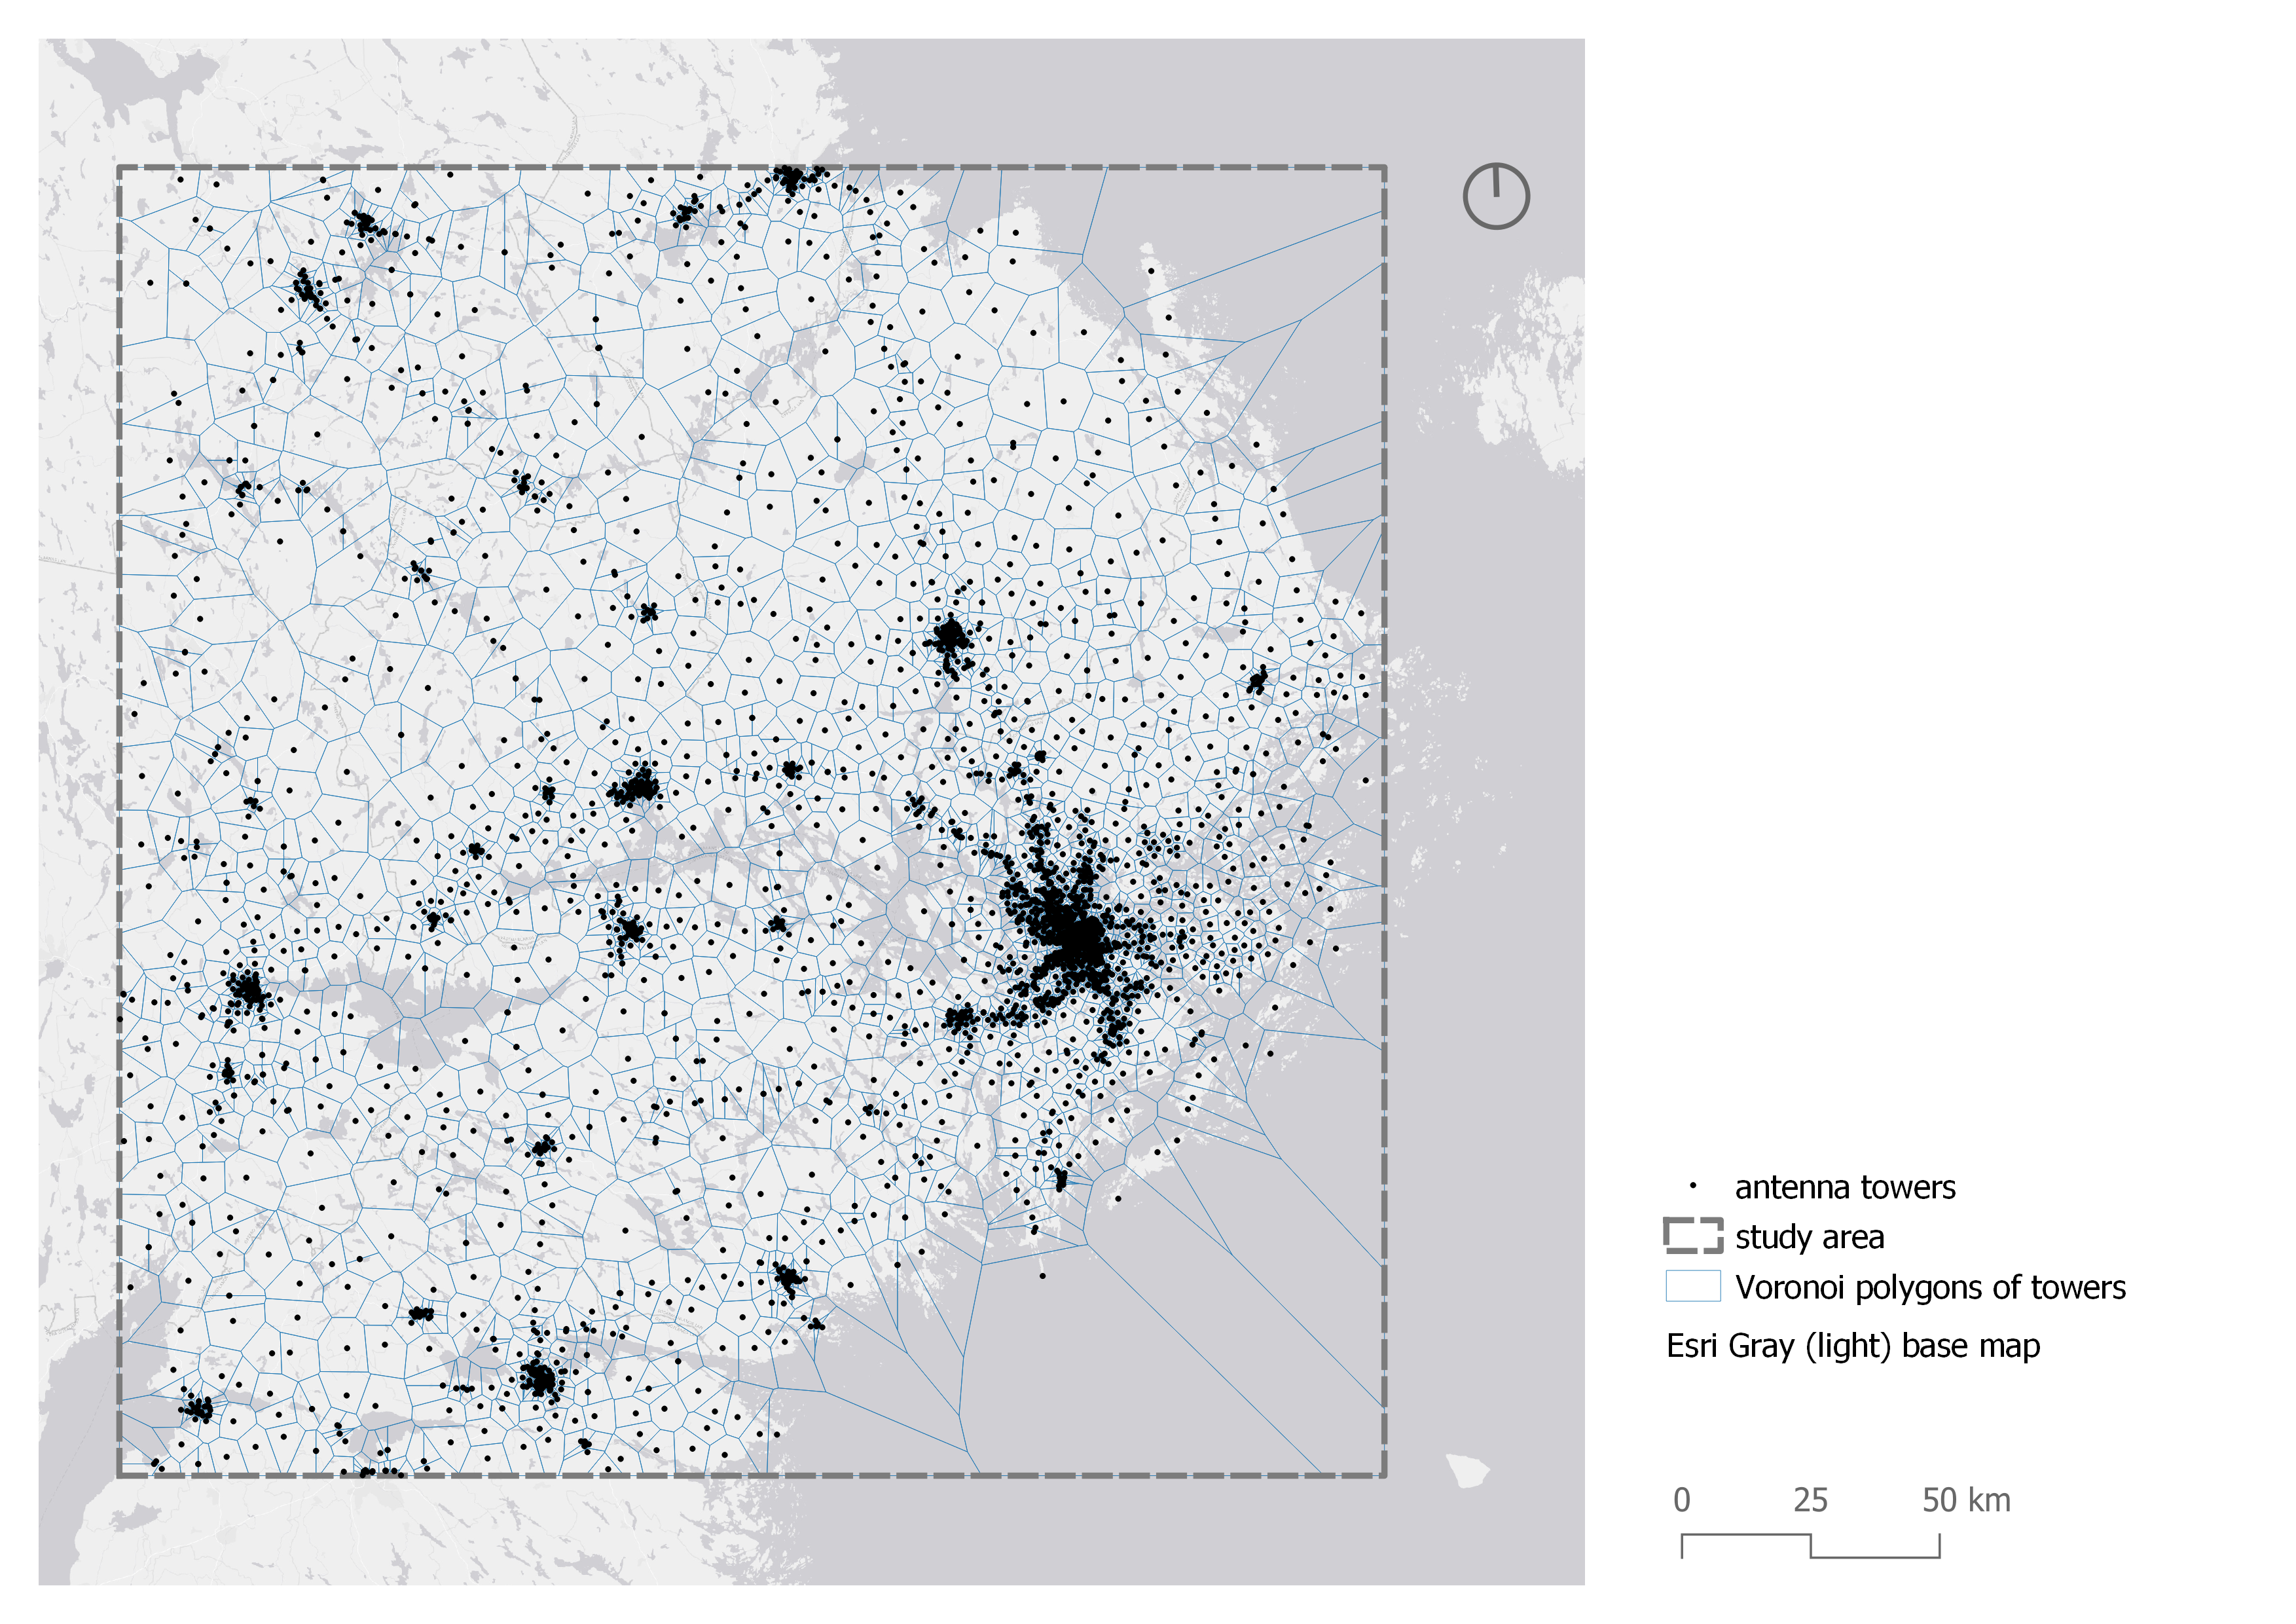
\includegraphics[width=14cm]{mpn_map.png}
  \caption{Voronoi diagram constructed for Uppsala and Stockholm's Mobile Phone Network}
  \label{fig:mpn_map}
\end{figure}


\subsubsection{Deterministic Trajectories under Voronoi Partition}
Assuming we are following this assumption, then trajectories and mobility patterns of our objects can be easily sketched. Here, we abstract it as a transition matrix, denoted as
\(\textbf{P}_0\). Using our sample data, a \(4,069 \times 4,069\) sparse matrix is constructed, where each transition is considered deterministic, from polygon \(m\) to \(n\). See Figure \ref{fig:determ_traj}.


\begin{figure}
  \centering
  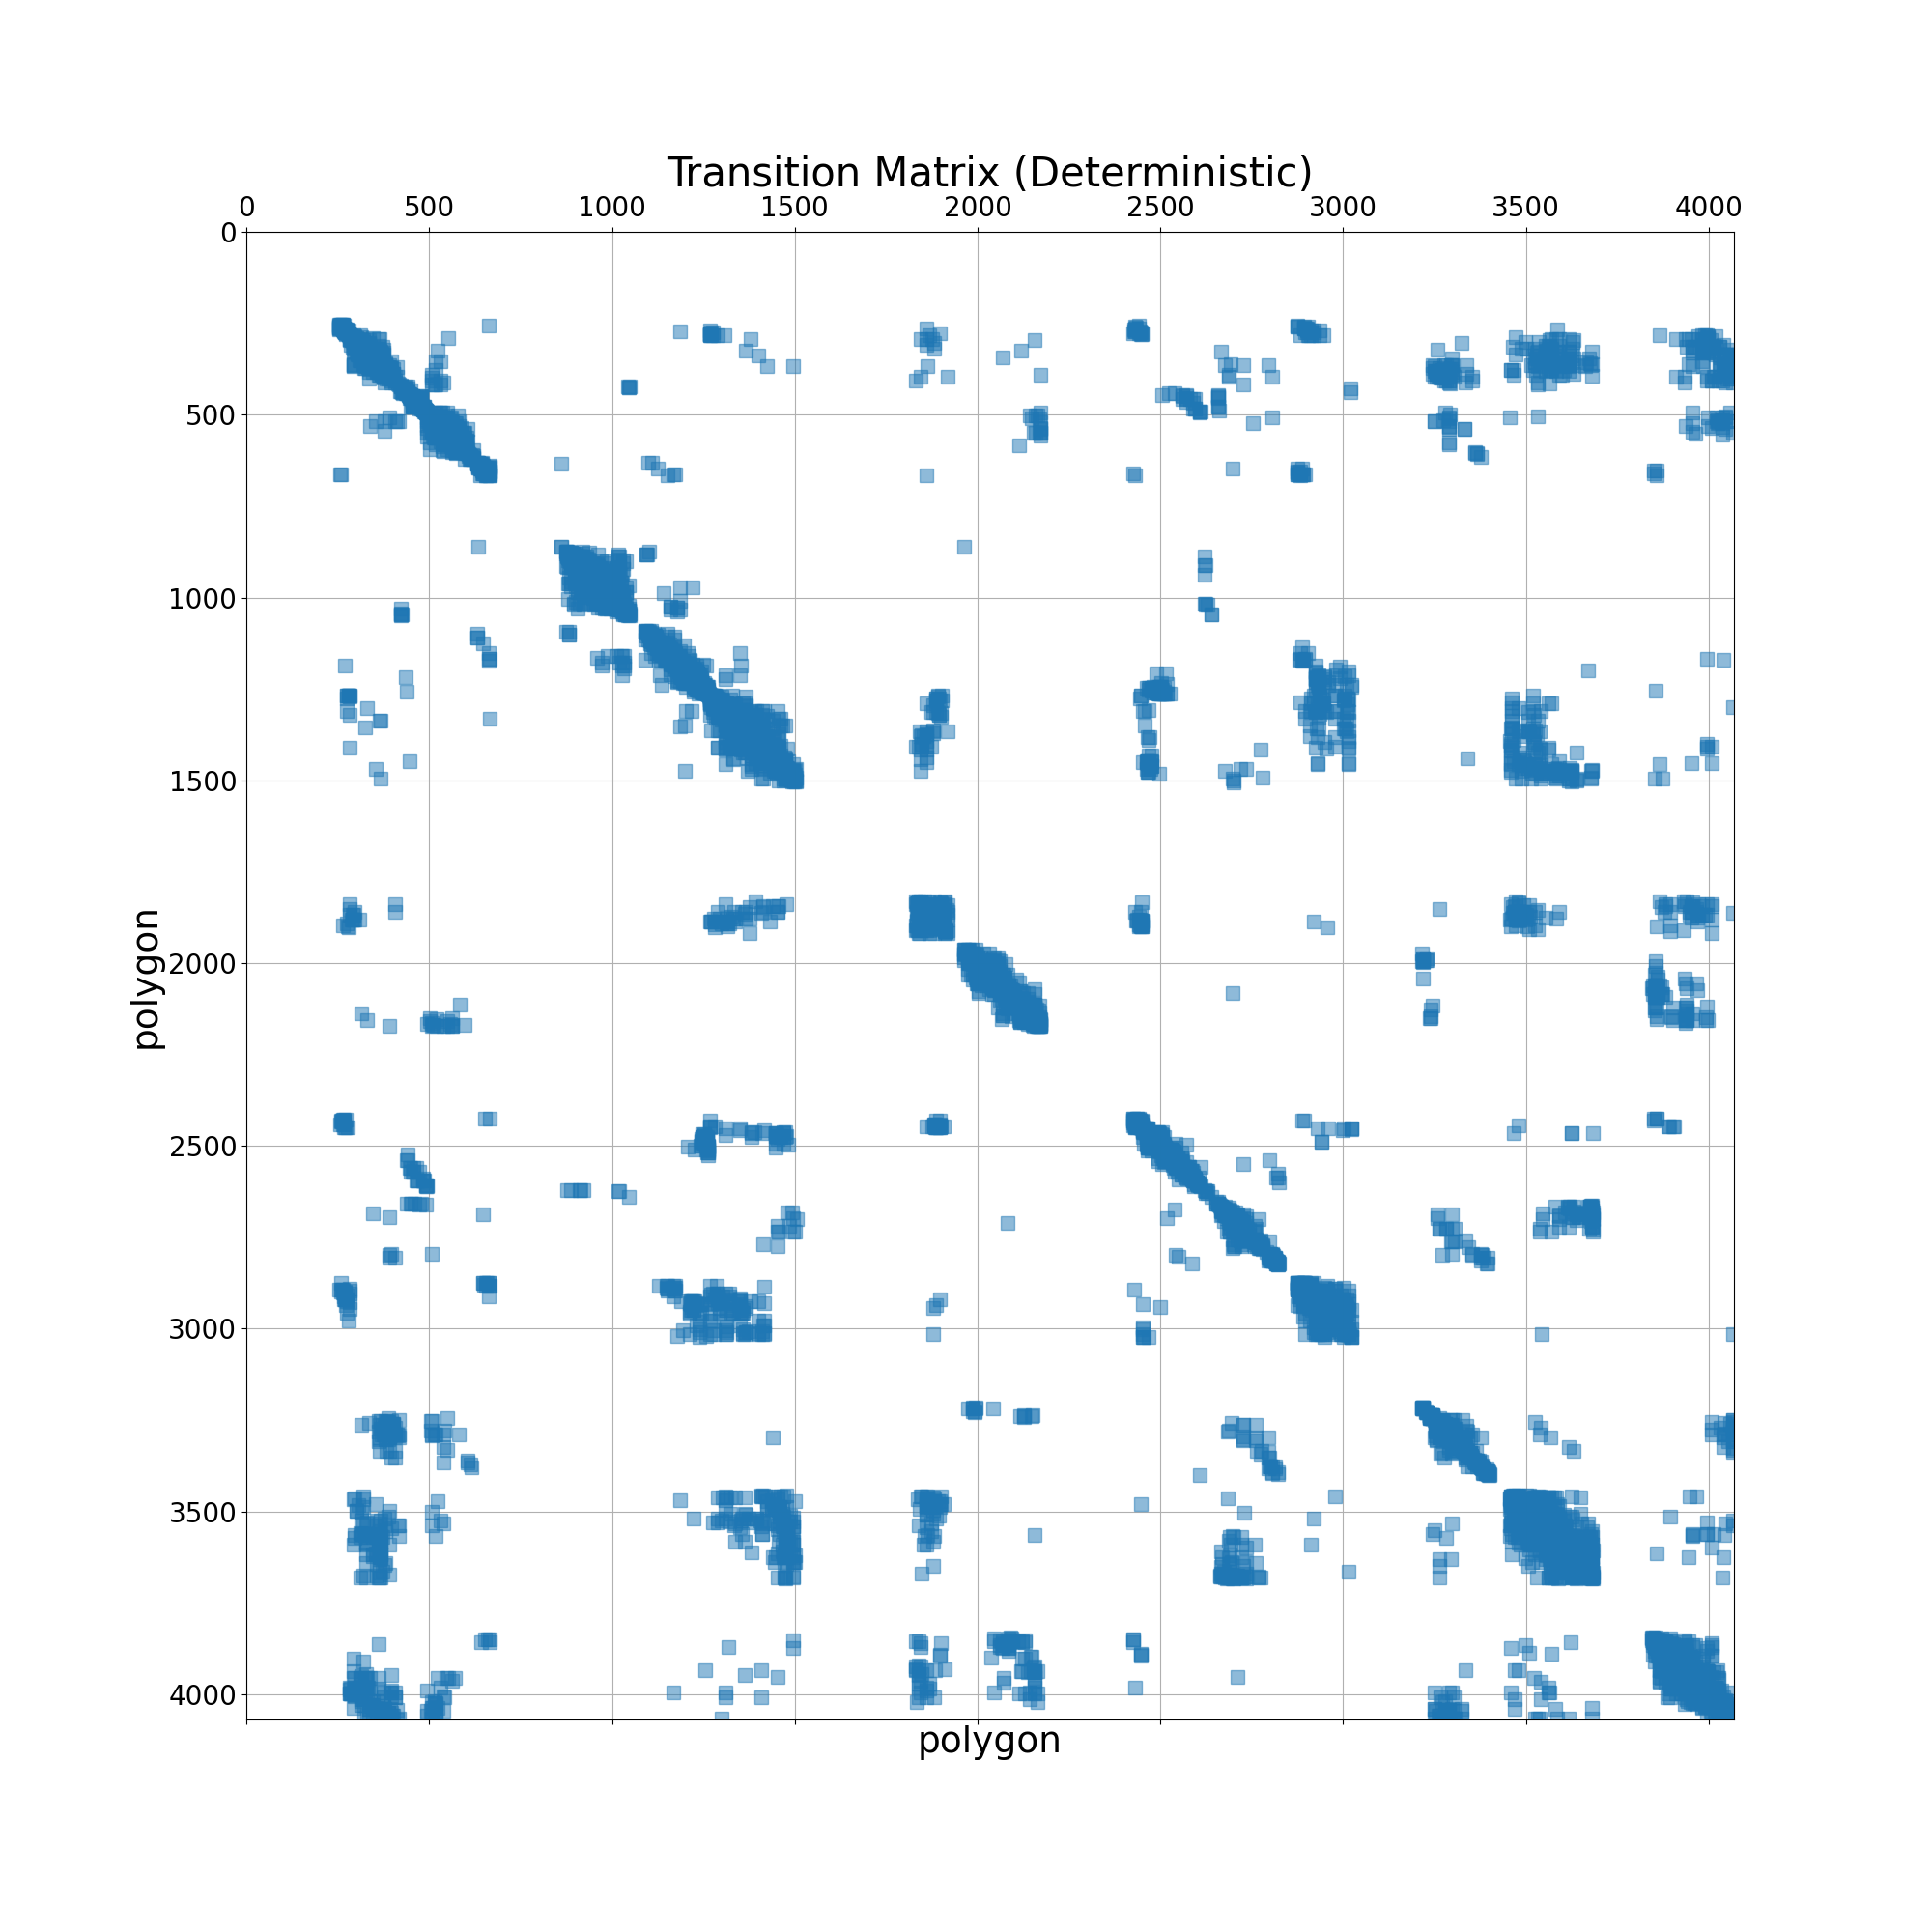
\includegraphics[width=8cm]{determ_traj.png}
  \caption{Deterministic transition matrix under Voronoi assumption}
  \label{fig:determ_traj}
\end{figure}


\subsubsection{The Fallacy of pure Voronoi Partition}
The above result relies greatly on the Voronoi tessellation assumption. However, this scheme has taken plenty of criticism these years due to the lack of high spatiotemporal resolution in this field. In 2010, the Bayesian Inference approach for positioning in Cellular Networks was developed. By incorporating more information such as the distance to the base station, the location of neighboring base stations, and levels of interference and noise, it improved 20\% accuracy compared with the baseline approach that users were uniformly distributed in Voronoi cell \cite{bayesian_inference_2010}. With the combination of Cell-level and Location Area-level data based on cell coverage maps, higher spatial accuracy has been achieved compared to Voronoi tessellation and cell tower locations \cite{interoperable_mpn_2016}. The Social and Economic Geography Department at Uppsala University, along with the Geography and Human Environment Department at Tel Aviv University, have also been doing a series of studies \cite{closest_antenna_fallacy_2021, prob_posit_mpn_2021}, to show how this presumption is faulty and developed more productive approaches in population density estimation, human mobility description, localization, etc.



This subsection will mostly explain the experimental results that Uppsala University and Tel Aviv University have obtained, by comparing GPS and MPN records that revealed their poor fit \cite{closest_antenna_fallacy_2021}. 


This experiment was implemented by measuring the distance between GPS location and the cell tower that served the device, with the help of a couple of volunteers who recorded their GPS trajectories. Figure \ref{fig:mc_connection}, which is from the referred research, demonstrates this scenario more intuitively. It records the cell towers located in its Voronoi cell during each time interval, and in the meanwhile, records other cell towers that actually served the device in both cases of connection with single cell tower and multiple cell towers during each time interval \cite{closest_antenna_fallacy_2021}.

\begin{figure}
  \centering
  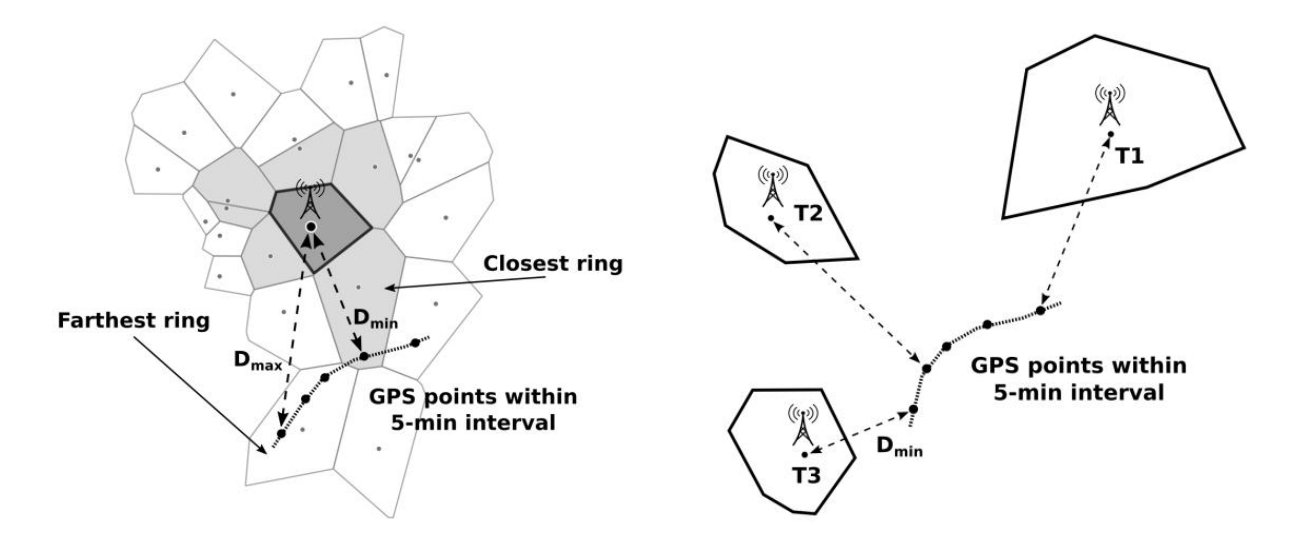
\includegraphics[width=12cm]{mc_connection.png}
  \caption{Distance between the mobile device and the cell towers served the device (multiple connections during 5-minute interval) \cite{closest_antenna_fallacy_2021}}
  \label{fig:mc_connection}
\end{figure}


\begin{figure}
  \centering
  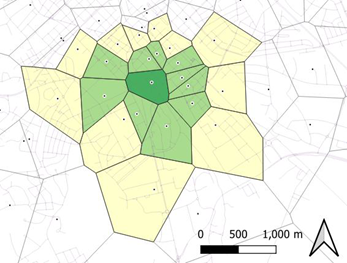
\includegraphics[width=8cm]{voronoi_ring.jpg}
  \caption{Voronoi cell with neighborhood rings of order 1 and 2 \cite{closest_antenna_fallacy_2021}}
  \label{fig:voronoi_ring}
\end{figure}

Another important element that needs to be noticed is the measurement of the distance. Aside from the standard method based on the Euclidean distance, which concluded that the average distance is 3,540 meters in their experiment, the measurement we will employ in this research is based on the adjacent ring neighborhoods of the Voronoi cell. In Figure \ref{fig:voronoi_ring}, the centered dark-green cell is considered as Voronoi cell itself that is the ring of order 0. Light-green cells are the neighboring rings of 1st order, and light-yellow cells can be seen as the 2nd order ring, etc. According to their experiment, the average distance in terms of the neighboring rings is 1.08 rings, and 63\% of connections are located beyond the Voronoi cell \cite{closest_antenna_fallacy_2021}. 



Their experiments showed the fallacy of pure Voronoi-based trajectories. In the next section, we proceed by applying some empirical statistics that their experiment concluded in order to generate distributed trajectories.



\subsection{Distributed Trajectories Generation: Voronoi Partition with Ring Distribution}
\label{sec:tm_voronoi_ring}
Under the Grid partition, we generated distributed trajectories by adding Gaussian noise on trajectories. While under the circumstance of Voronoi partition, we analogize this procedure with empirical statistics from the above experiments. Since the distance between GPS location and the served cell tower can be measured as the unit of rings, the empirical statistics we will use is the distribution of ring distance, as shown in Figure \ref{fig:ring_distance}.

\begin{figure}
  \centering
  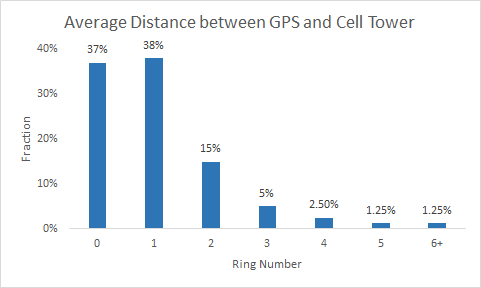
\includegraphics[width=12cm]{ring_distance.jpg}
  \caption{Average distance between the location of the device and the cell tower: in terms of rings \cite{closest_antenna_fallacy_2021}}
  \label{fig:ring_distance}
\end{figure}

The algorithm for adding noise on trajectories under Voronoi partition is given next.


\begin{algorithm}
  \caption{Algorithm for adding noise on trajectories under Voronoi partition}
  \label{alg:ring-noise}
  \begin{algorithmic}
    \Procedure{EmpiricalRing}{$x^{(t)},y^{(t)}$}
    \Comment{parameters: current coordinate}
    \State \textbf{Transformation} \(pol^{(t)} \gets (x^{(t)},y^{(t)})\) \Comment{pol represents polygon ID}
    \State \(p_{pol^{(t)},0} \gets Fraction_{[0]}\) \Comment{assign order 0 empirical prob to polygon}
    \For{\(RingOrder_{[i]}, i \in \{1,2,3,4,5,6\}\)}
    \State \textbf{Count} \(N_{pol^{(t)},i}\) \Comment{number of adjacent neighbors}
    \State \textbf{Enumeration} \(M_{pol^{(t)},i,j}\) \Comment{members of adjacent neighbors}
    \State \Comment{\(\sum_{j}{\left| M_{pol^{(t)},i,j} \right|}=N_{pol^{(t)},i}\)}
    \State \(p_{pol^{(t)},i} \gets Fraction_{[i]}/N_{pol^{(t)},i}\) \Comment{assign order i empirical prob}
    \EndFor
    \EndProcedure
  \end{algorithmic}
\end{algorithm}


As the empirical statistics indicate, pure Voronoi partition has only 37\% credibility, while after the first ring is accounted for, 75\% percentile could be reached, 90\% after the second, and 95\% after the third, etc. Under this framework, we demonstrate the whole dynamics of distributed trajectories once again in the form of transition matrix \textbf{P}. Transition matrix \textbf{P}, in this case, can be expressed as:
\begin{equation*}
    \textbf{P}=\sum_{n}\sum_{t}(\boldsymbol{v}_{n}^{(t)})(\boldsymbol{v}_{n}^{t+1})^{T}.
\end{equation*}


Since each user’s trajectories are independent of each other, by assumption, \(n\) represents the number of independent users. By the logic of Algorithm \ref{alg:ring-noise}, for each user in each timestamp, their recorded location, aka their state \(s \in \mathbb{S}\), would be vectorized as a distribution \(\boldsymbol{v}\). \(\boldsymbol{v}\), in this case, is a \(4,069 \times 1\) vector, and \(\boldsymbol{v}^{T}\) is its transpose. Noted:
\begin{equation*}
    \{\sum_{j=1}^{4,069} v_{i,j}^{(t)}:\{0.37,0.75,0.90,0.95,0.975,0.9875,1\},
    i=\{0,1,2,3,4,5,6\},v_{i,j}^{(t)} \in \boldsymbol{v}^{(t)} \},
\end{equation*}

where \(i\) represents the number of rings considered. In order to make it a probability, we need to normalize each vector \(\boldsymbol{v}\) for a given ring order \(i\):

\begin{equation*}
    \{\sum_{j=1}^{4,069} v_{i,j}^{(t)}=1, i=\{0,1,2,3\}, v_{i,j}^{(t)} \in \boldsymbol{v}^{(t)} \},
\end{equation*}

so that empirical statistics, in this case, would represent its confidence level. Therefore, with 1st, 2nd, and 3rd ring accumulatively taken into account (here we stopped at ring order 3), their respective transition matrix \(\textbf{P}_i\) is constructed (See Figure \ref{fig:tm_1}, \ref{fig:tm_2}, \ref{fig:tm_3}).

\newpage

\begin{figure}
  \centering
  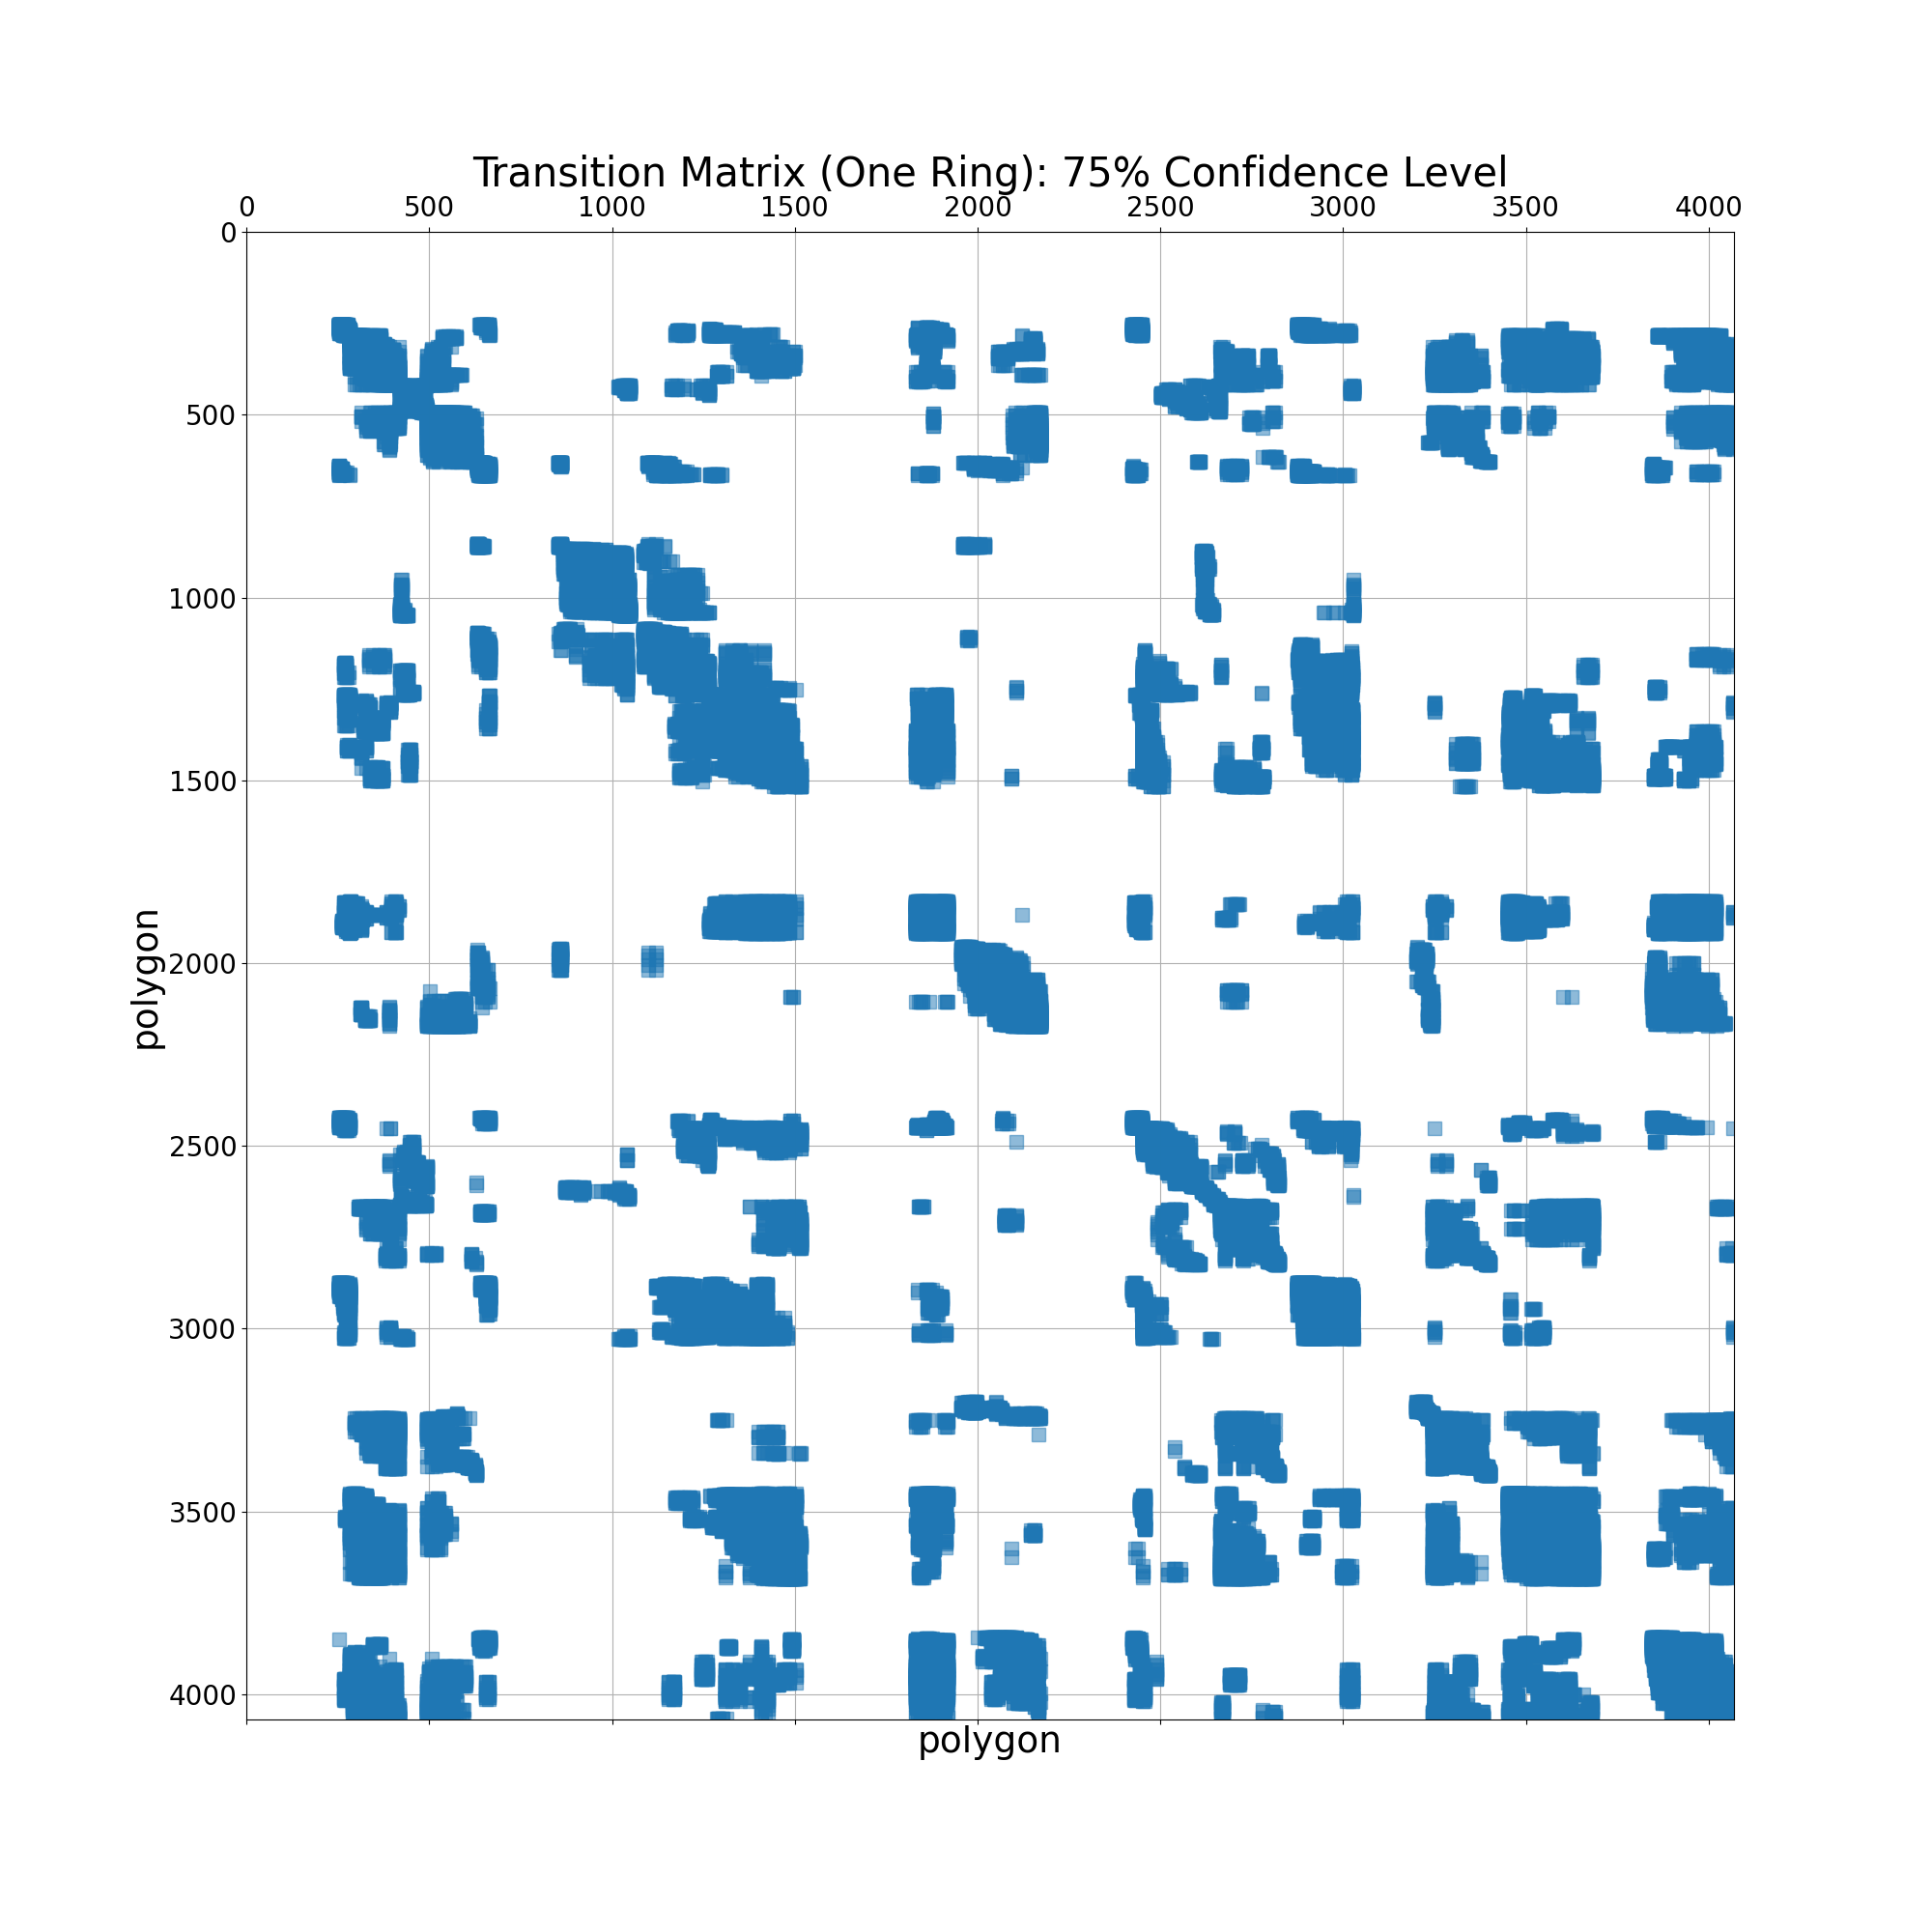
\includegraphics[width=8cm]{TM_1.png}
  \caption{Transition matrix with one ring noise}
  \label{fig:tm_1}
\end{figure}

\begin{figure}
  \centering
  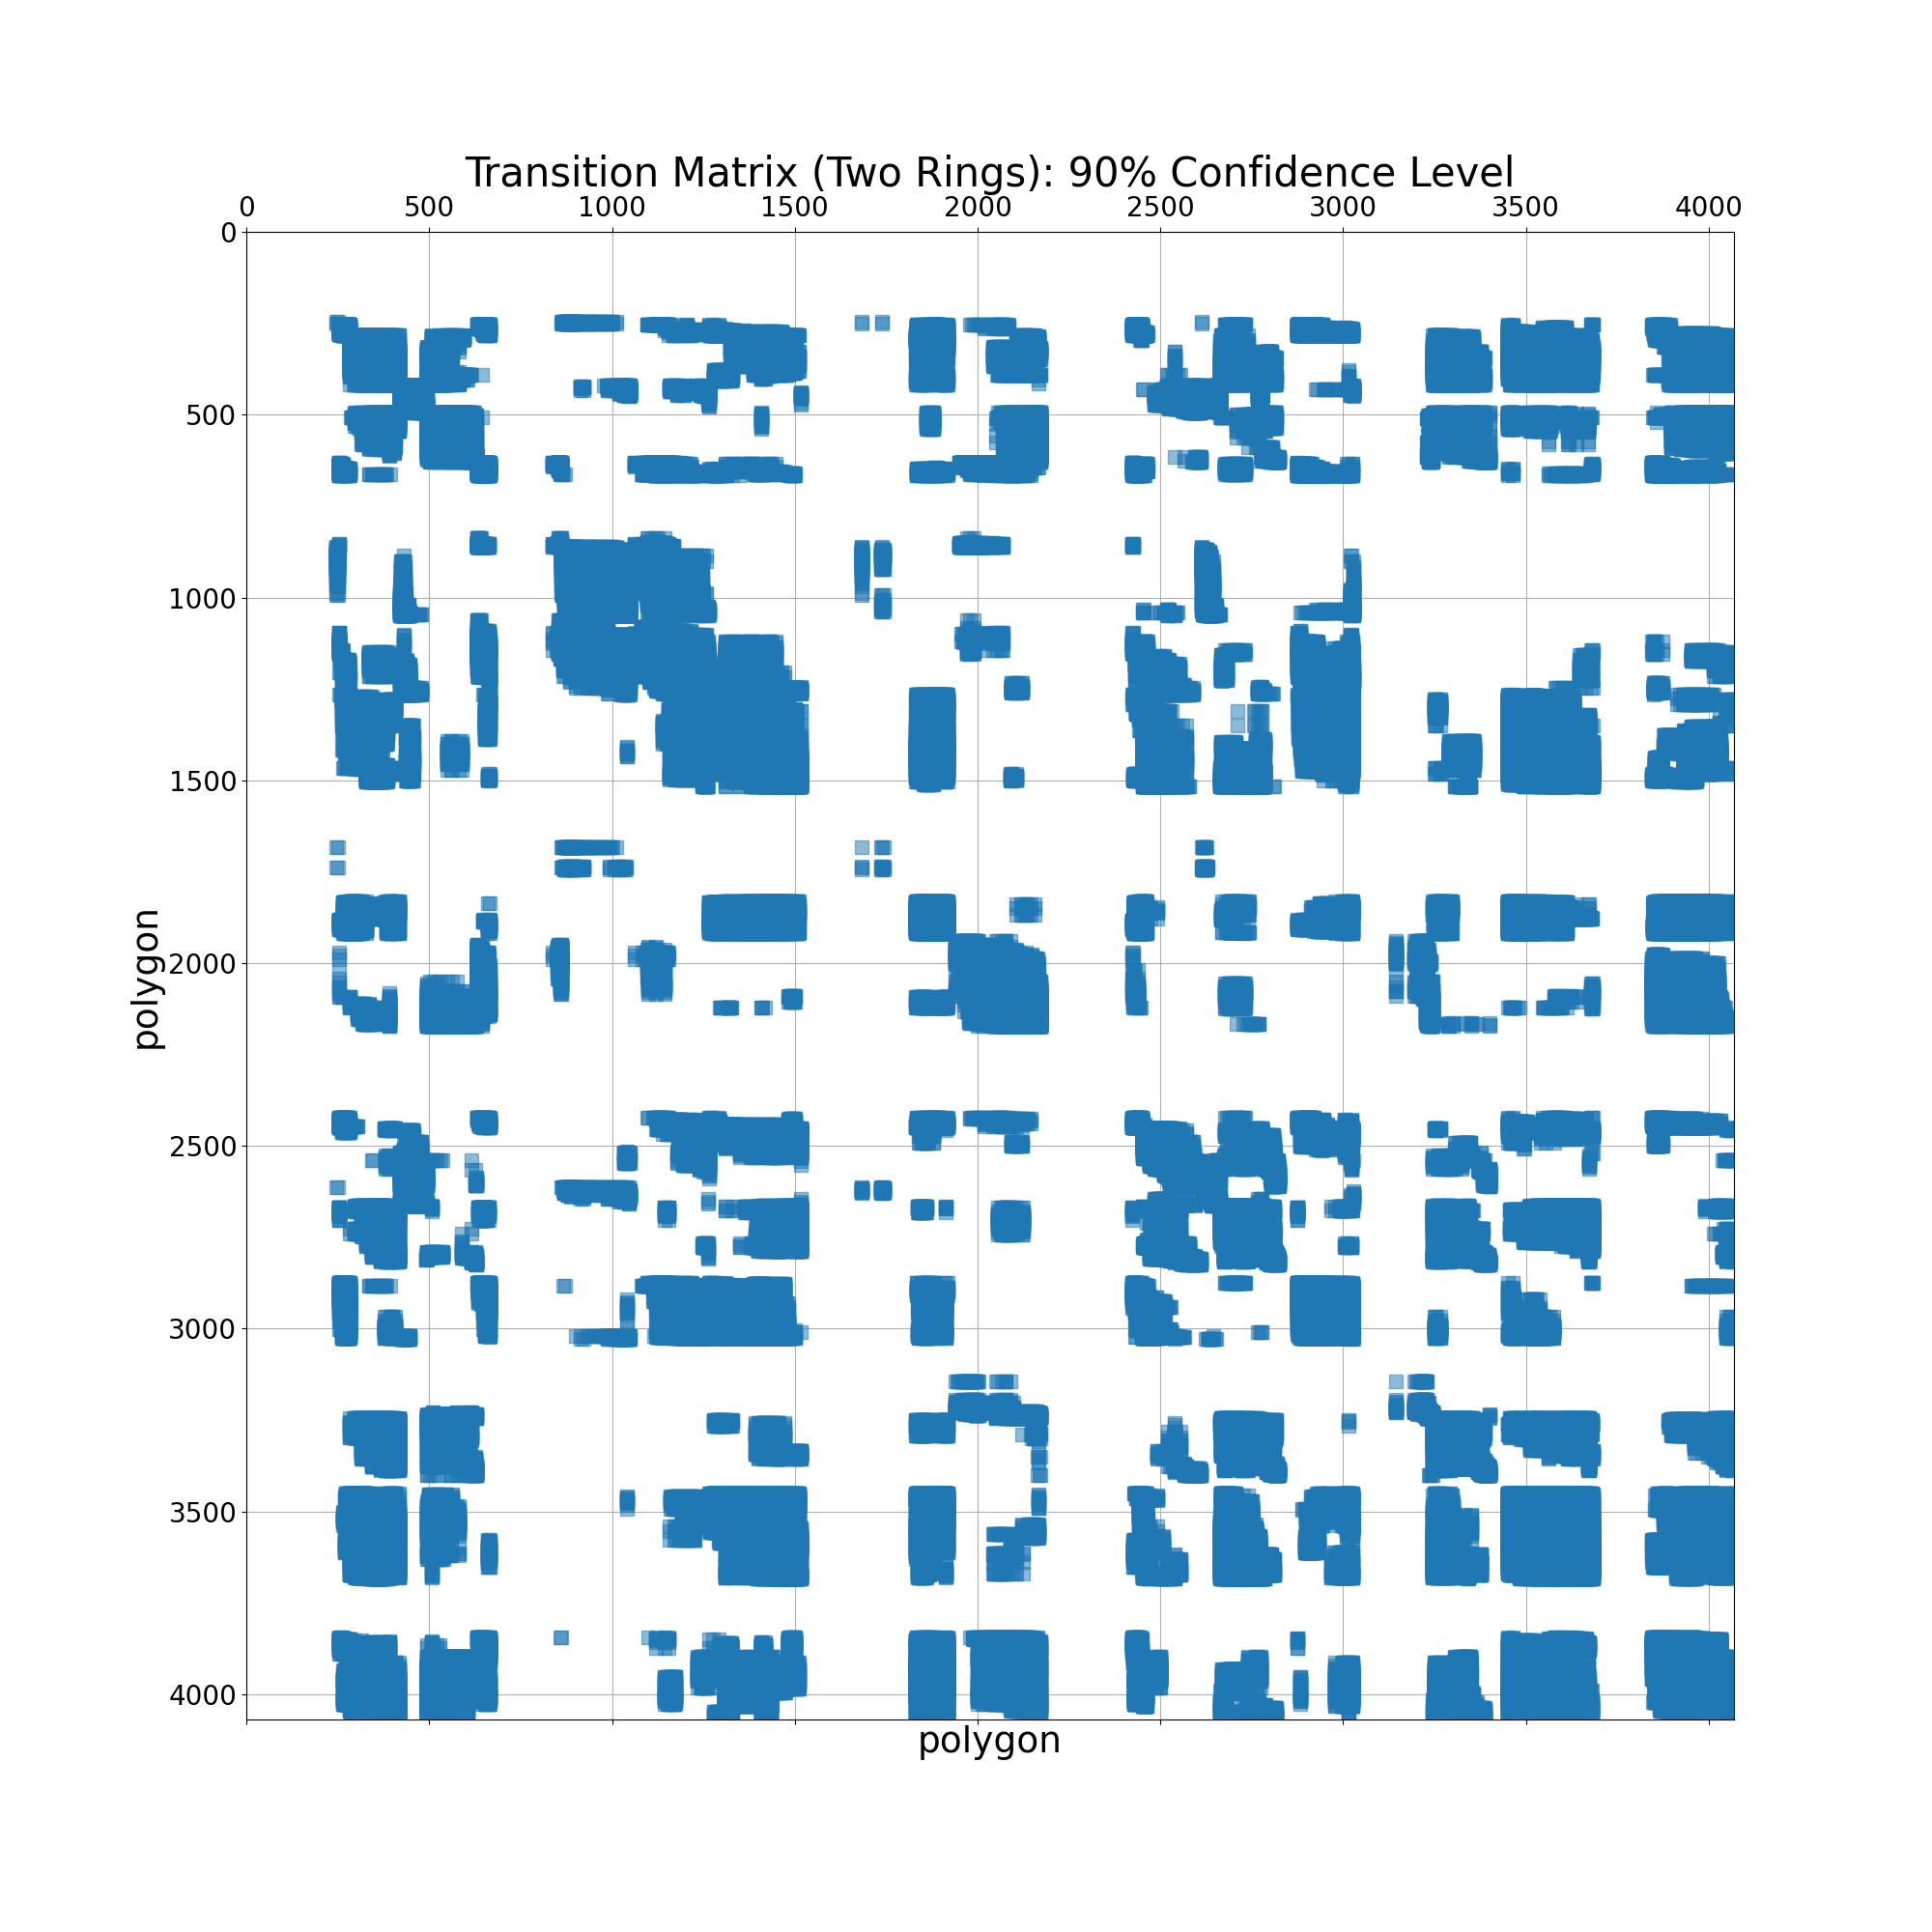
\includegraphics[width=8cm]{TM_2.png}
  \caption{Transition matrix with two rings noise}
  \label{fig:tm_2}
\end{figure}




\begin{figure}
  \centering
  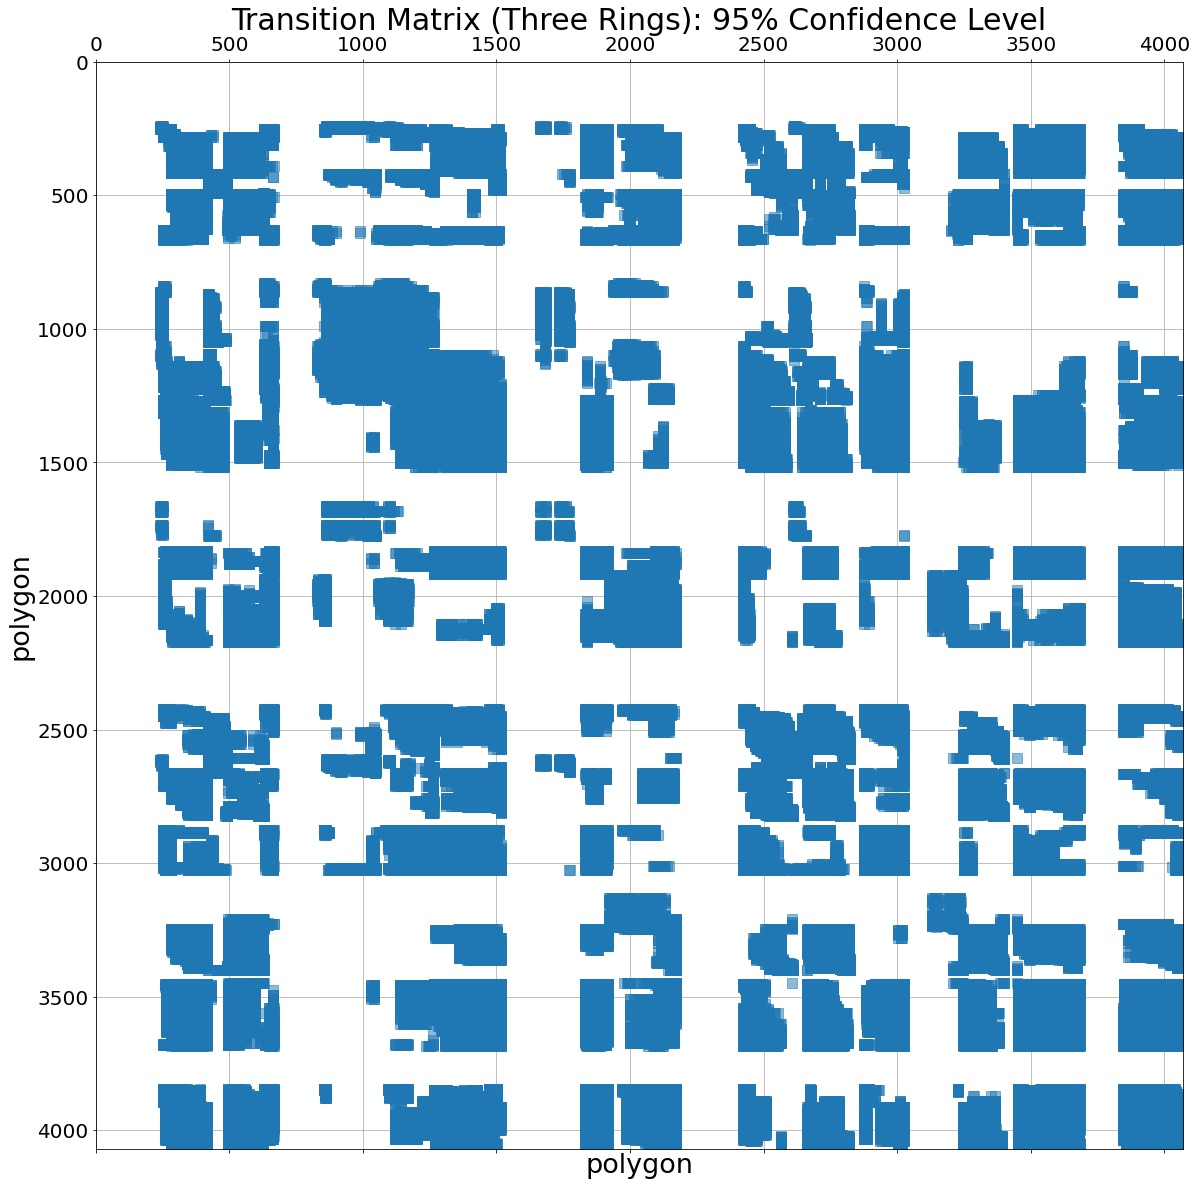
\includegraphics[width=6.7cm]{TM_3.png}
  \caption{Transition matrix with three rings noise}
  \label{fig:tm_3}
\end{figure}


It is evident that as more rings are considered, meaning more noises added to the original mobile data, the matrix goes from sparse to dense, thus generating more potential locations where objects might have been. This is another way of trade-off between bias and variance. In order to make results more meaningful, we transform the above plots into the probabilistic point of view so that each transition can be aggregated into probability values. We take the first ring noise as an example. See Figure \ref{fig:tm_prob}, which is transformed from Figure \ref{fig:tm_1} (For computational efficiency purposes, in the following sections, we also consider the first ring only).



\begin{figure}
  \centering
  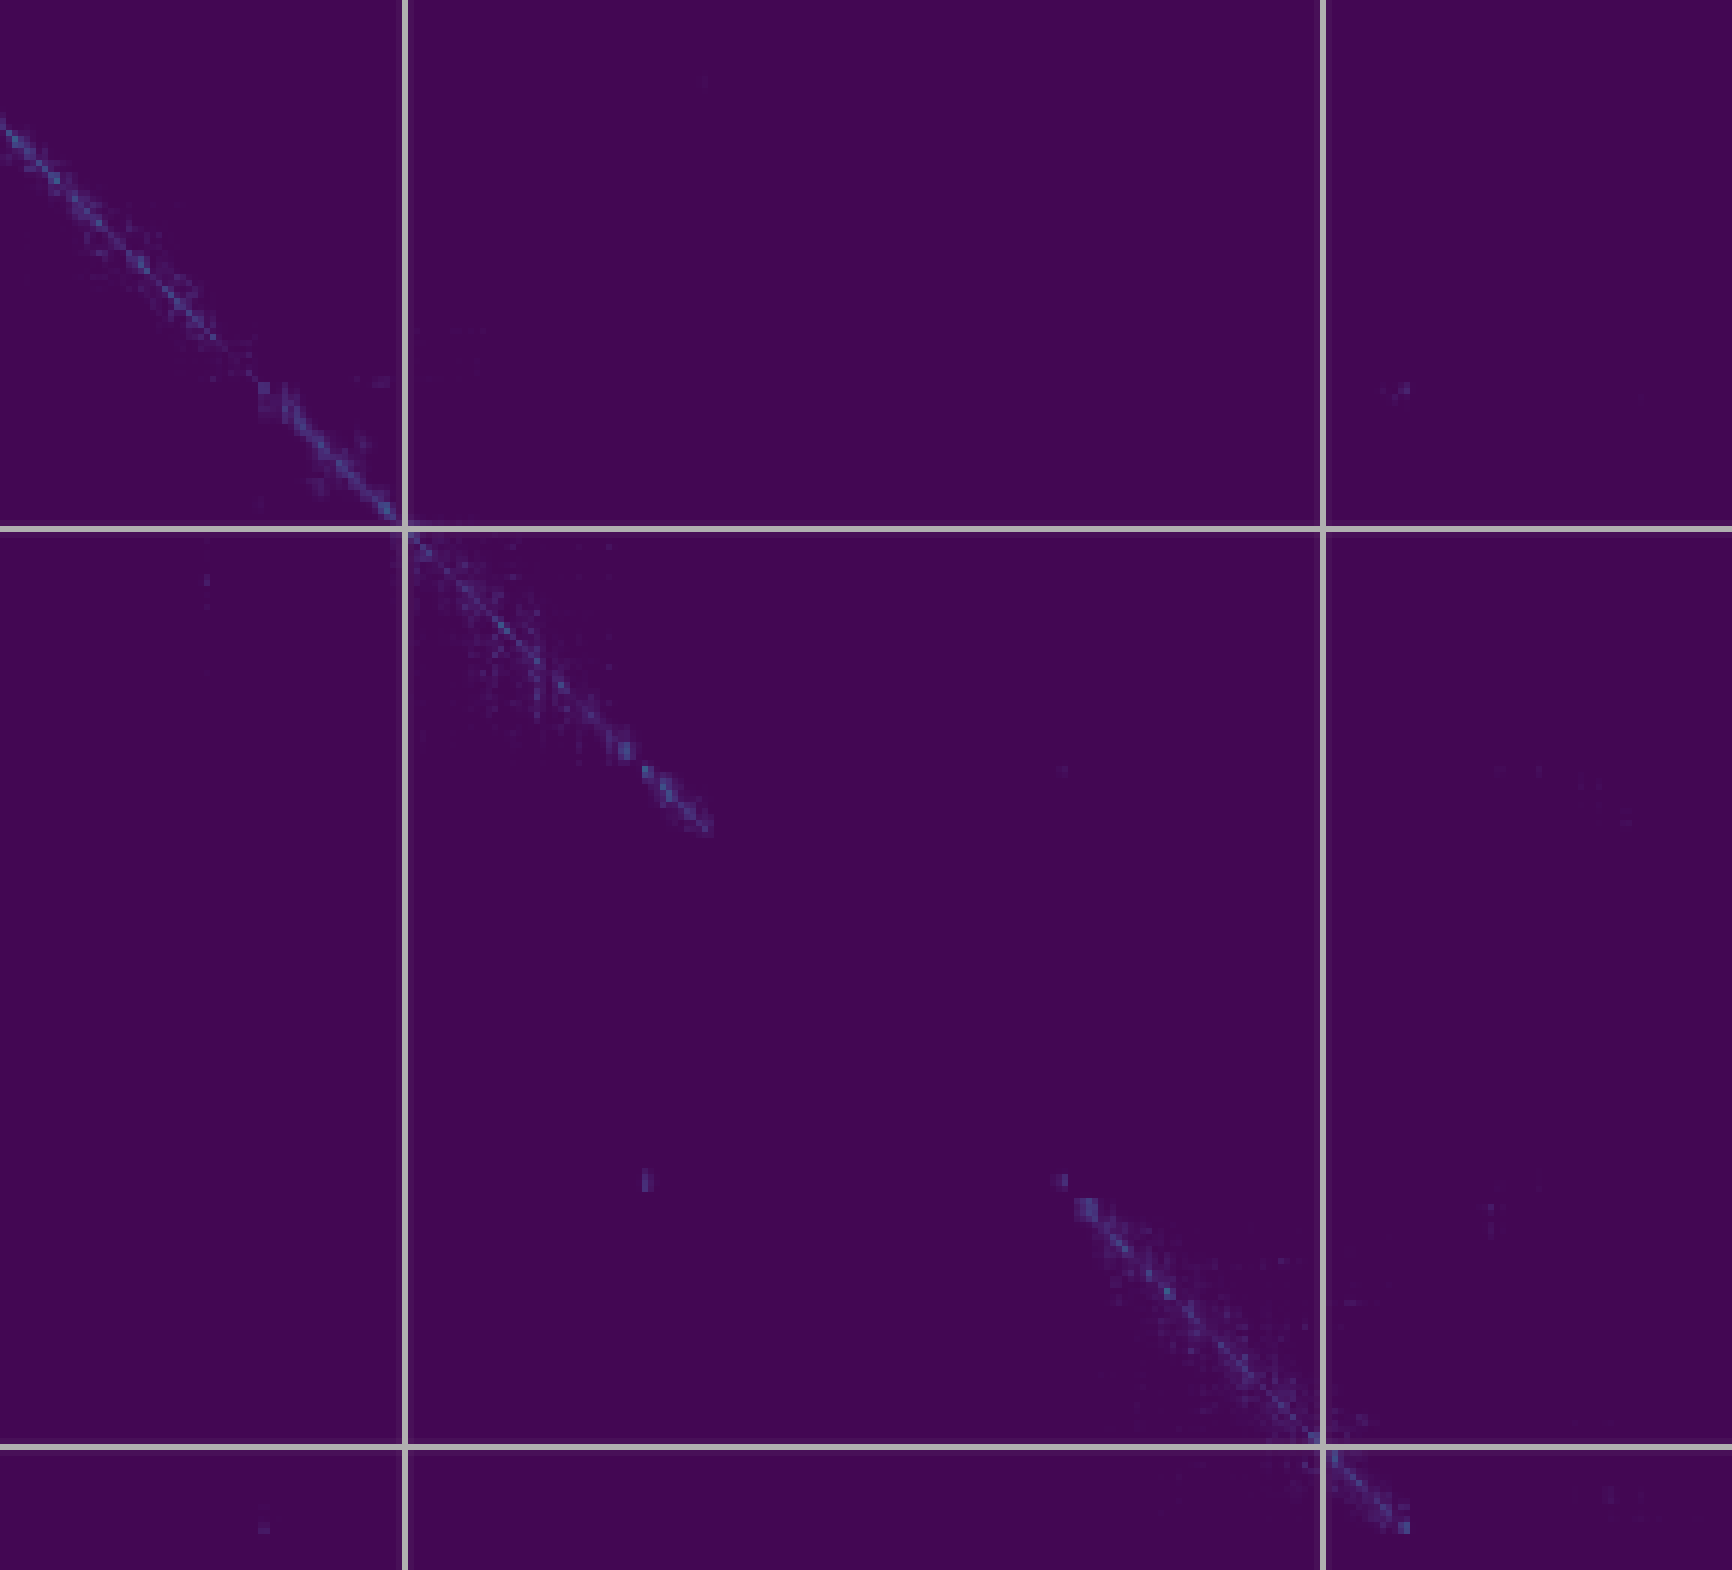
\includegraphics[width=8cm]{TM_1_probs.png}
  \caption{Transition matrix from probabilistic point of view}
  \label{fig:tm_prob}
\end{figure}
\newpage


According to Figure \ref{fig:tm_prob} \footnote{In our sample, we only have 1,000 objects but 4,069 locations, which means too few people for too broad a space, causing the result to be very sparse. Due to this limitation, we zoom in on this plot and only cut out a piece of it to have a more clear visualization.}, the transition matrix in a full-time period tends to be diagonal in shape, which corresponds to Figure \ref{fig:determ_traj}. When considering trajectories to be deterministic, the mobility seems to be more diagonal and sparse than the sequence from Figure \ref{fig:tm_1} to Figure \ref{fig:tm_3} that progressively added more noise. Moreover, it also indicates most people would remain still most of the time, especially after periods of working and sleeping are considered, which also corresponds to the habitual nature of their behavior.  \newpage




%=========================================================%





\section{Distributed Trajectories under Voronoi-Ring Framework}
It is worthy to notice that observing mobility trends with the full-time transition matrix, even in a big dataset, may not be ideal. The periods of working and sleeping make up a large proportion of daily life, which inevitable interfere the whole picture. In this section, we overcome this predicament by constructing alternative abstractions to display the trend of mobility/trajectories more feasibly and dynamically, using Origin-Destination (OD) matrix and Time-inhomogeneous matrix.


\subsection{Origin-Destination Matrix}
Origin-destination (OD) matrix is a matrix in which each element represents the number of trips from the origin (\(i\)) to the destination (\(j\)). It is a routine way of depicting the transportation system. Automatically generated data, or sensing data, such as Automatic Vehicle Location (AVL) systems, Global Positioning System (GPS), and Mobile Phone Network (MPN), are becoming active in constructing OD matrix due to their time-efficiency, cost-friendliness, and accuracy. One prevalent type of research for OD matrix construction is based on the taxi trajectory data. According to the study from the Civil Engineering Department at the University of Calgary, their methodology for taxi pick-up and drop-off detection based on service status information and origin and destination clustering with X-means algorithm, portrayed the traffic flows situation of Lisbon \cite{od_taxi_2019}. There is also established existing research in OD matrix construction in the mobile area. In 2013, Md. Shahadat Iqbal et al. implemented this with aggregated CDR, which contains IDs, duration, and spatiotemporal information, and combined it with traffic counts data extracted from video recordings to offset the segments when users did not use their phones \cite{od_mpn_2014}. 

The methodologies for OD matrix construction are various, depending on the available resources. In our project, we plan to construct OD matrix based on the current framework, with MPN data and the structure we built for transition matrix \textbf{P} in section \ref{sec:tm_voronoi_ring}. 


A transition matrix \textbf{P} in our case was constructed as:
\begin{equation*}
    \textbf{P}=\sum_{n}\sum_{t}(\boldsymbol{v}_{n}^{(t)})(\boldsymbol{v}_{n}^{t+1})^{T},
\end{equation*}

each \boldsymbol{v} is a normalized vector based on the empirical distribution of ring distance (see Figure \ref{fig:ring_distance}), such that: 

\begin{equation*}
    \{\sum_{j=1}^{4,069} v_{i,j}^{(t)}=1, i=\{0,1,2,3,4,5,6\}, v_{i,j}^{(t)} \in \boldsymbol{v}^{(t)} \}.
\end{equation*}

However, the main drawback of this representation is that it is statical. Numerous transitions are redundant since they are meant to be still. One effective way of improving this is to consider the time interval. During this time interval, we assume their trajectories are mobilized; even not, we can categorize their origins and destinations as identical, which is still valuable. Based on this framework, OD matrix can be easily constructed:

\begin{equation*}
    \textbf{OD}=\sum_{n}\sum_{t}(\boldsymbol{v}_{n}^{(t-h)})(\boldsymbol{v}_{n}^{t+h})^{T},
\end{equation*}

where \(h\) represents the time interval, the only variation compared to transition matrix \textbf{P}. 


Figure \ref{fig:od} (a) demonstrates the Origin-Destination matrix with time interval \(h\) set as 2 hours, which means we assume their trajectories will be updated within 4 hours in this case; and Figure \ref{fig:od} (b) is the transition matrix with one ring noise, from Figure \ref{fig:tm_1}.

Let us compare Figure \ref{fig:od} (a) with Figure \ref{fig:od} (b), where both cases considered first order of ring, but whose shapes vary significantly. This illustrates the difference between periodicity and sequentiality. For the OD matrix, mobility was considered in a time span instead of an instant moment. Regardless of how big or small the probability is for each point in this case, the OD matrix is more suitable for sketching the mobility pattern over a longer time scale.


\begin{figure}
  \centering
  \begin{subfigure}[t]{0.45\textwidth}
    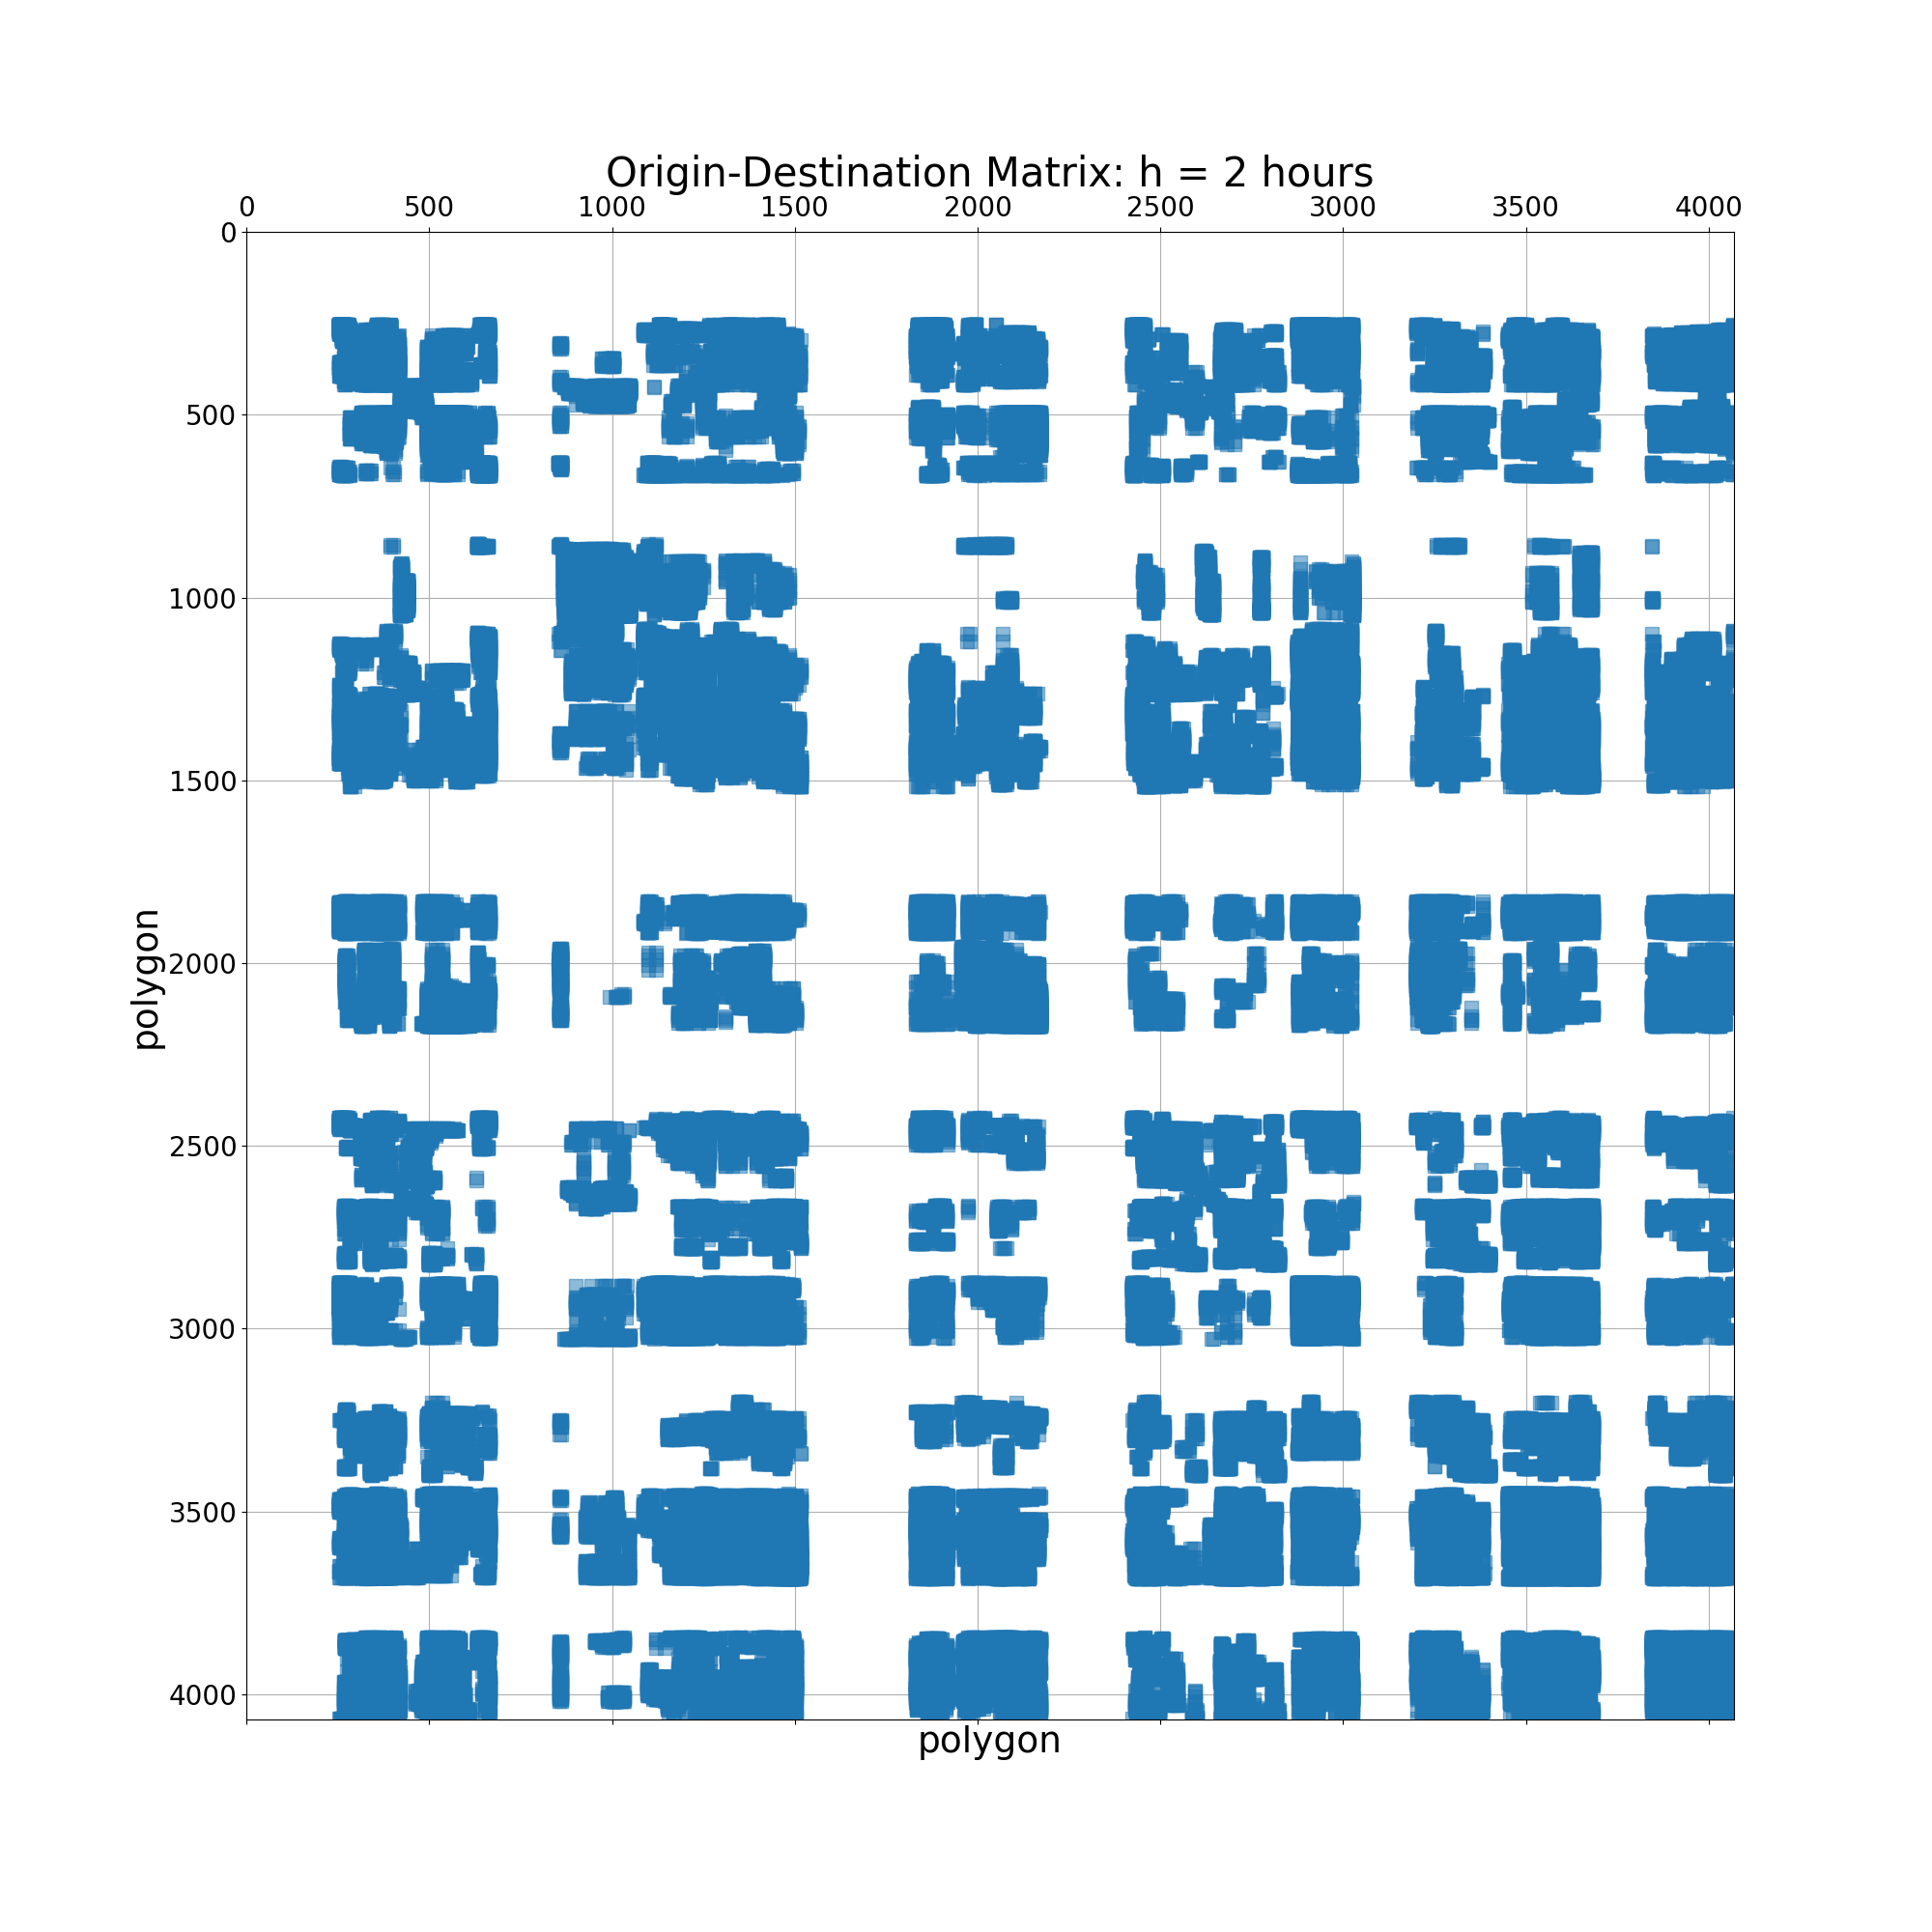
\includegraphics[width=\textwidth]{OD.png}
    \caption{}
  \end{subfigure}
  \begin{subfigure}[t]{0.45\textwidth}
    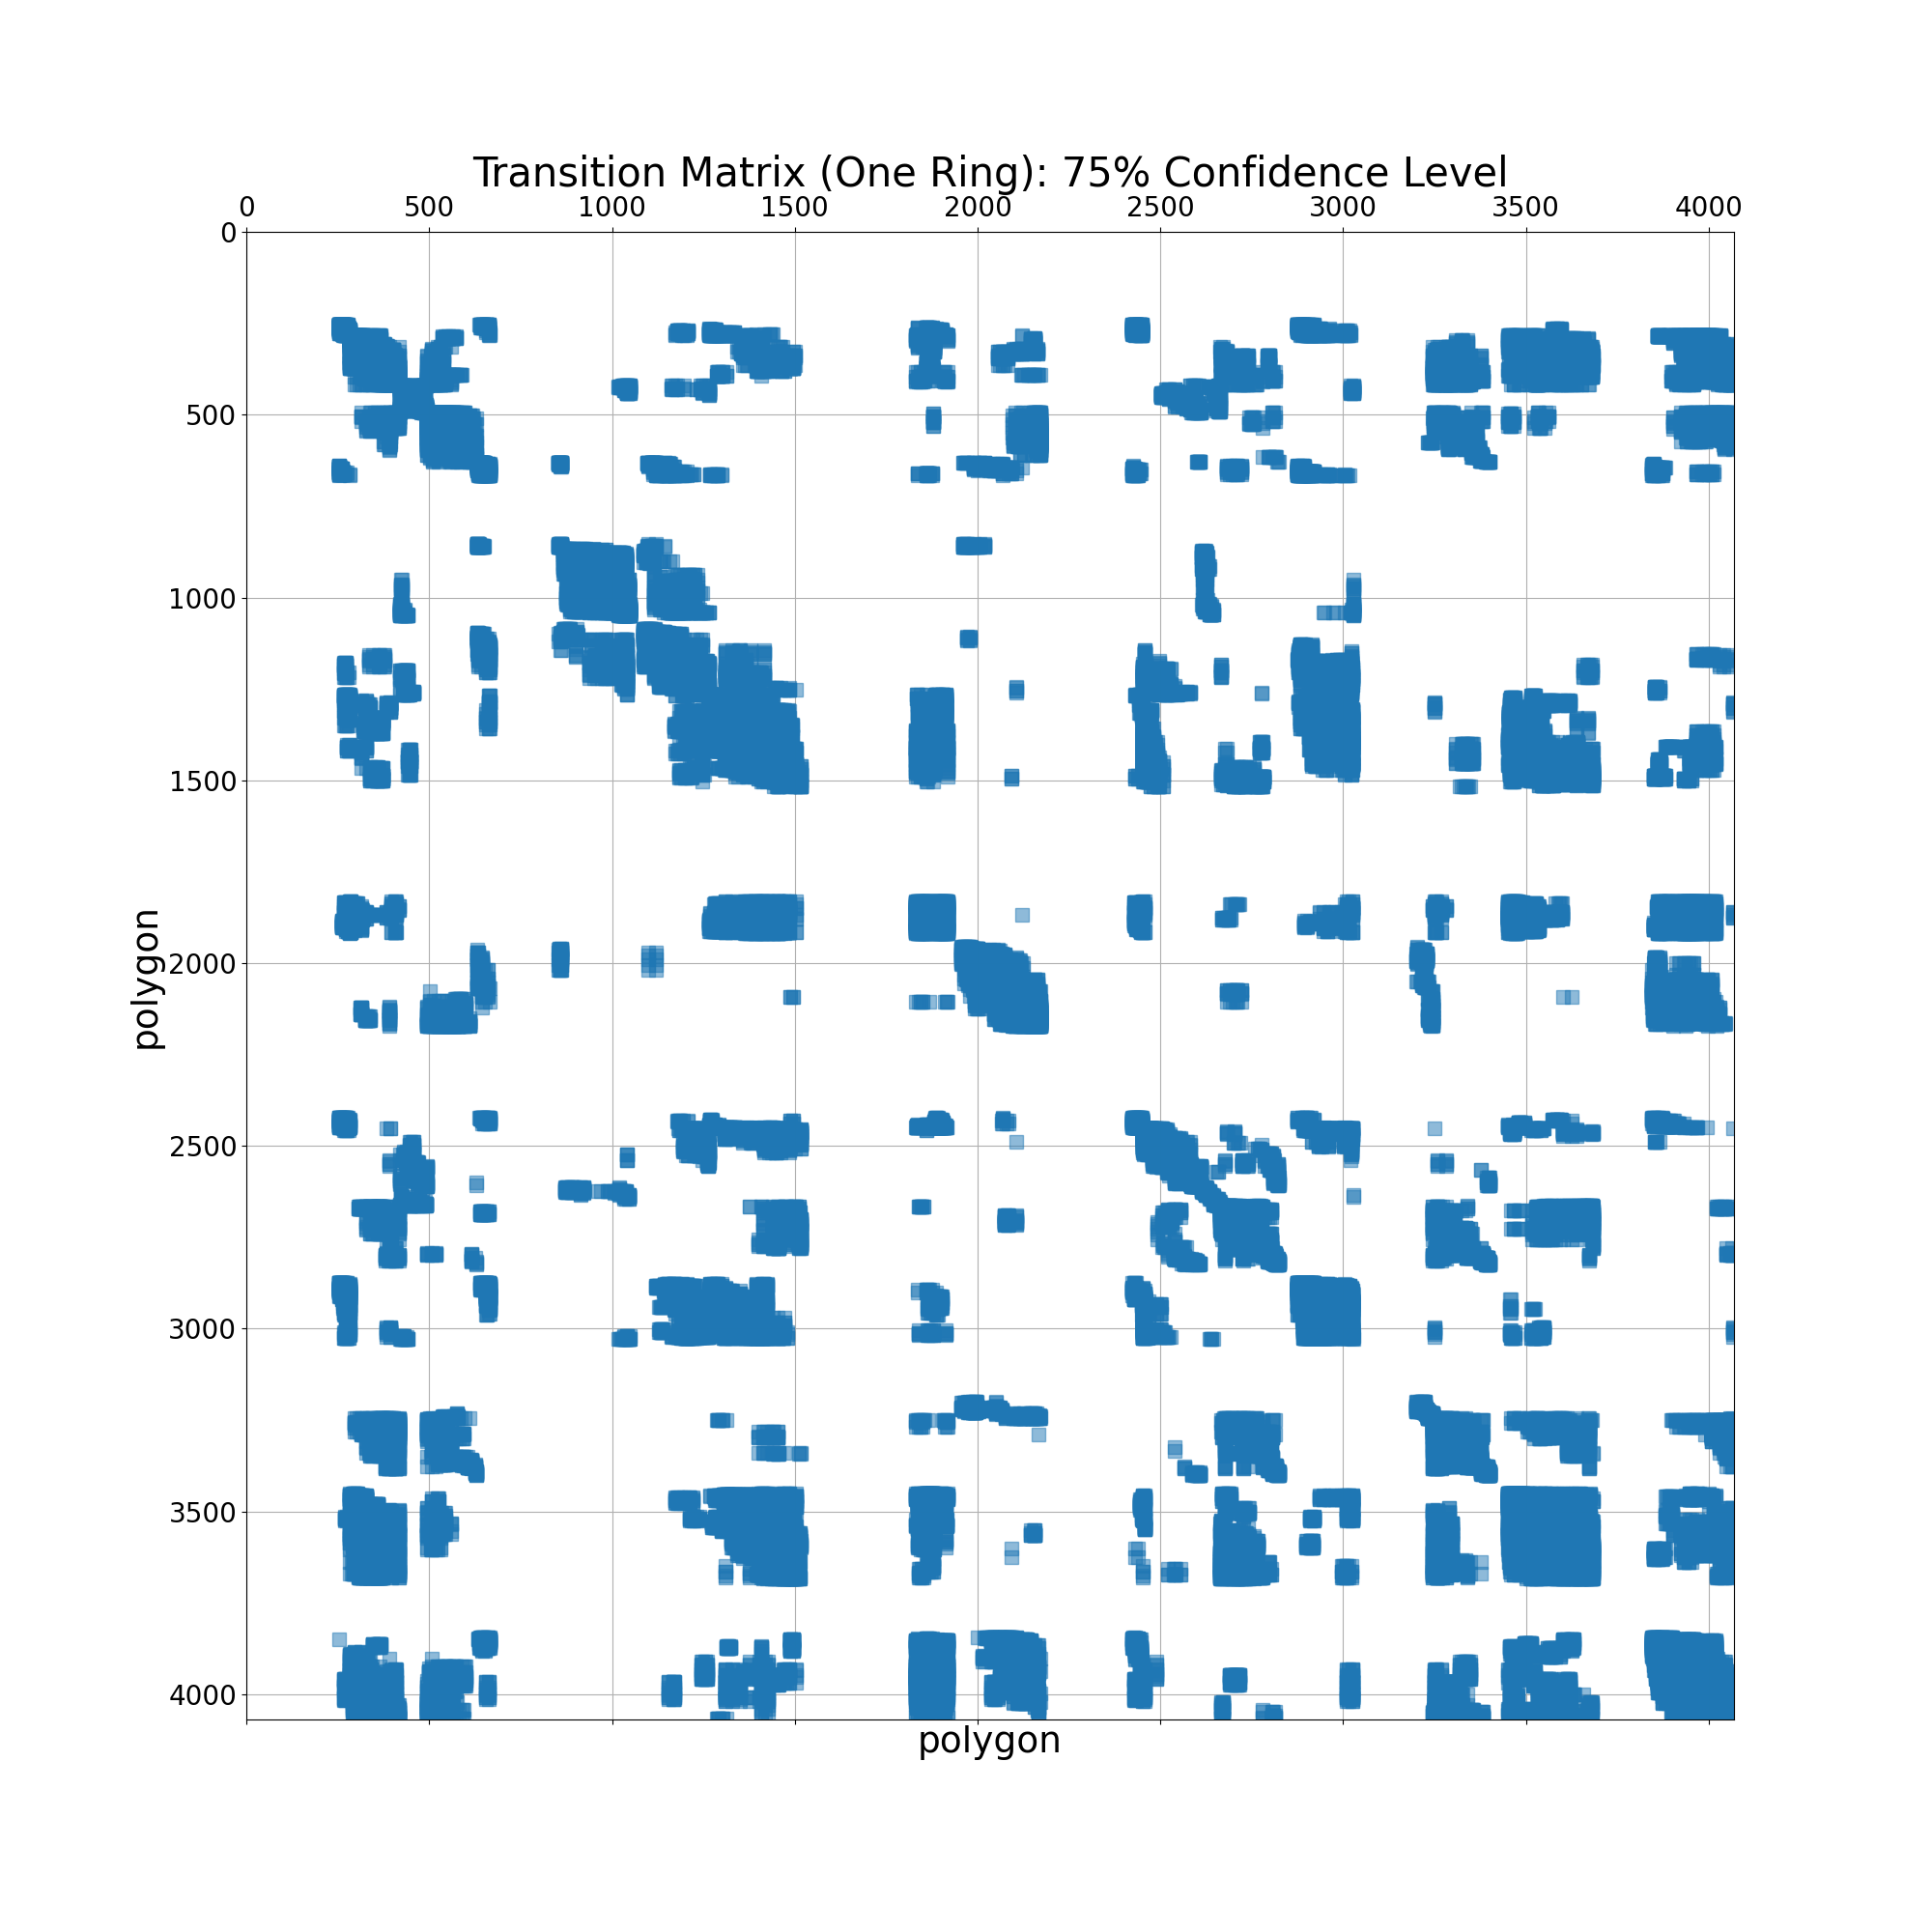
\includegraphics[width=\textwidth]{TM_1.png}
    \caption{}
  \end{subfigure}

  \caption{Comparison between Origin-Destination matrix and transition probability matrix, with one ring noise}
  \label{fig:od}
\end{figure}



\subsection{Time-inhomogeneous Matrix}
The transition matrix \textbf{P} was earlier constructed under the assumption of time-homogeneity, which is not accurate when we want to allow for variation in transitions between different time intervals. For a more realistic model, we consider transition matrix \textbf{P} to be time-inhomogeneous, which means the transition probabilities \(p_{i,j}\) depend on time. Below we give the formal definitions of time-homogeneous and time-inhomogeneous Markov chain on a finite state space.


\begin{definition}[\textbf{Time-homogeneous Markov chain}]
\label{def:time_homo_markov_chain}
A Markov chain \((X_{t})_{t \geq 0}\) is time-homogeneous if:
\begin{equation*}
P(X_{2}=j|X_{1}=i)=P(X_{3}=j|X_{2}=i)=...=P(X_{t+1}=j|X_{t}=i),
\end{equation*}
where the transition probabilities \(p_{i,j}=P(X_{t+1}=j|X_{t}=i) \) does not depend on time \(t\), and transition matrix \(\textbf{P}:=\{p_{i,j}\}_{i,j \in \mathbb{S}}\) is constant or homogeneous for all time \(t\).
\end{definition}



\begin{definition}[\textbf{Time-inhomogeneous Markov chain}]
\label{def:time_inhomo_markov_chain}
A Markov chain \((X_{t})_{t \geq 0}\)  is time-inhomogeneous if the transition probabilities \(p_{i,j}\) depend on time \(t\), that is:
\begin{equation*}
p_{t,i,j}:=P(X_{t+1}=j|X_{t}=i),
\end{equation*}
and the matrix:
\begin{equation*}
\textbf{P}_{(t)}:=\{p_{t,i,j}\}_{i,j \in \mathbb{S}}, 
\end{equation*}
represents the transition probability matrix at time \(t\).
\end{definition}

A time-inhomogeneous matrix from time \(m\) to \(n\) can be expressed as:
\begin{equation*}
    \textbf{P}_{(m,n)}=\textbf{P}_{(m)} \times \textbf{P}_{(m+1)} \times ... \times \textbf{P}_{(n)} (n>m>0) \; \cite{markov_chain_2020}
\end{equation*}

Once we regard the transition matrix \textbf{P} as time-inhomogeneous, we can make divisions on \textbf{P} into a series of sub-transition matrix \(\textbf{P}_{(i)}\) for specific analytical purposes. For example, if we only pay attention to the transition matrix from 2 am to 3 am, there is no doubt that it will be displayed with a significant diagonal shape since most people sleep during that period. On the contrary, if we consider the transition matrix from 7 am to 9 am on weekdays, the shape will be less diagonal but more dispersed because of the morning rush hour.

The division on \textbf{P} does not have to be of equal length. We can divide \textbf{P} empirically, as we assumed above that transition matrices between 2 am to 3 am, and 7 am to 9 am are very likely to be different. Or we can measure their difference using standard norms, such as:
\begin{equation*}
    \textbf{L}_{2}(\textbf{P}_{(x)},\textbf{P}_{(y)})={\left\lVert \textbf{P}_{(x)}-\textbf{P}_{(y)}\right\rVert}_{2,1}=\textstyle \sum_{j=1}^{\left| \mathbb{S} \right|} {\left\lVert p_{j}\right\rVert}_{2}=\textstyle \sum_{j=1}^{\left| \mathbb{S} \right|} (\textstyle \sum_{i=1}^{\left| \mathbb{S} \right|}  {\lvert p_{i,j} \rvert}^2)^{1/2}.
\end{equation*}


\newpage


%=========================================================%






\section{Time-inhomogeneous Simulation}
\label{sec:ti_sim}
The above techniques we developed can be implemented for multiple uses. One common application, especially for areas such as mobility trends, population density, traffic control, etc., is usually associated with forecasting. With the MPN records at a certain time, we can vectorize such information as a distribution at this moment; plus, the above matrices we constructed can be regarded as empirical models. We will take these as entry points for further analysis in this section. 



\subsection{Stationary Distribution}
\label{sec:stationary}
When it comes to vectors and matrices, one simple application is stationary distribution. The stationary distribution of the Markov chain is a probability distribution that remains steady as time progresses, represented as a vector \(\boldsymbol{\pi}\), with \(\textstyle \sum_{j=1}^{\left| \mathbb{S} \right|} {\pi}_{j} =1\). Given the transition matrix \textbf{P}, \(\boldsymbol{\pi}\) satisfied the following:
\begin{equation*}
    \boldsymbol{\pi}=\boldsymbol{\pi} \times \textbf{P}.
\end{equation*}


From the forecasting point of view, we can intercept the latest MPN records and vectorize them as an initial vector \(\boldsymbol{v}_{0}\). By raising the transition matrix \textbf{P} to the power of iteration times:
\begin{equation*}
    \boldsymbol{v}_{1}=\boldsymbol{v}_{0} \times \textbf{P}
\end{equation*}
\begin{equation*}
   \boldsymbol{v}_{2}=\boldsymbol{v}_{1} \times \textbf{P}=\boldsymbol{v}_{0} \times \textbf{P}^{2}
\end{equation*}
\begin{equation*}
   ......
\end{equation*}
\begin{equation*}
   \boldsymbol{v}_{n}=\boldsymbol{v}_{n-1} \times \textbf{P}=...=\boldsymbol{v}_{0} \times \textbf{P}^{n}=\boldsymbol{\pi}, \text{as} \: n \to \infty
\end{equation*}

If \(\boldsymbol{\pi}=\boldsymbol{\pi} \times \textbf{P}\), then \(\boldsymbol{\pi}\) is the stationary distribution of the Markov chain.


With the idea of the time-inhomogeneous transition matrix, we can separate a transition matrix \textbf{P} into several sub-transition matrices \(\textbf{P}_{(m)}\), \(\textbf{P}_{(m+1)}\), \(\textbf{P}_{(m+2)}\), etc., observe if the initial vector \(\boldsymbol{v}_{0}\) will converge to the stationary distribution, and compare the initial vector \(\boldsymbol{v}_{0}\) and stationary distribution \(\boldsymbol{\pi}_{i}\)  at a different stage to view its mobility trend. See below:

\begin{equation*}
    \boldsymbol{\pi}_{1}=\boldsymbol{v}_{0} \times \textbf{P}_{(0)}^{n_{0}}
\end{equation*}
\begin{equation*}
   \boldsymbol{\pi}_{2}=\boldsymbol{\pi}_{1} \times \textbf{P}_{(1)}^{n_{1}}
\end{equation*}
\begin{equation*}
   ......
\end{equation*}
\begin{equation*}
   \boldsymbol{\pi}_{N}=\boldsymbol{\pi}_{N-1} \times \textbf{P}_{(N-1)}^{n_{N-1}}
\end{equation*}

In this case, we empirically select two transition matrices at two different stages that are assumed to be different, which are 8 am to 9 am and 9 am to 10 am. We intercept the latest MPN records that is at 8 am and vectorize them as the initial vector \(\boldsymbol{v}_{0}\). By implementing the above steps, firstly, we observe both vectors converge to the stationary distribution after 150 and 50 iterations, respectively, then we compare these two vectors along with stationary distribution to view this as a mobility trend. (See Figure \ref{fig:convergence_test}, \ref{fig:mob_trend}).


\begin{figure}
  \centering
  \begin{subfigure}[t]{0.8\textwidth}
    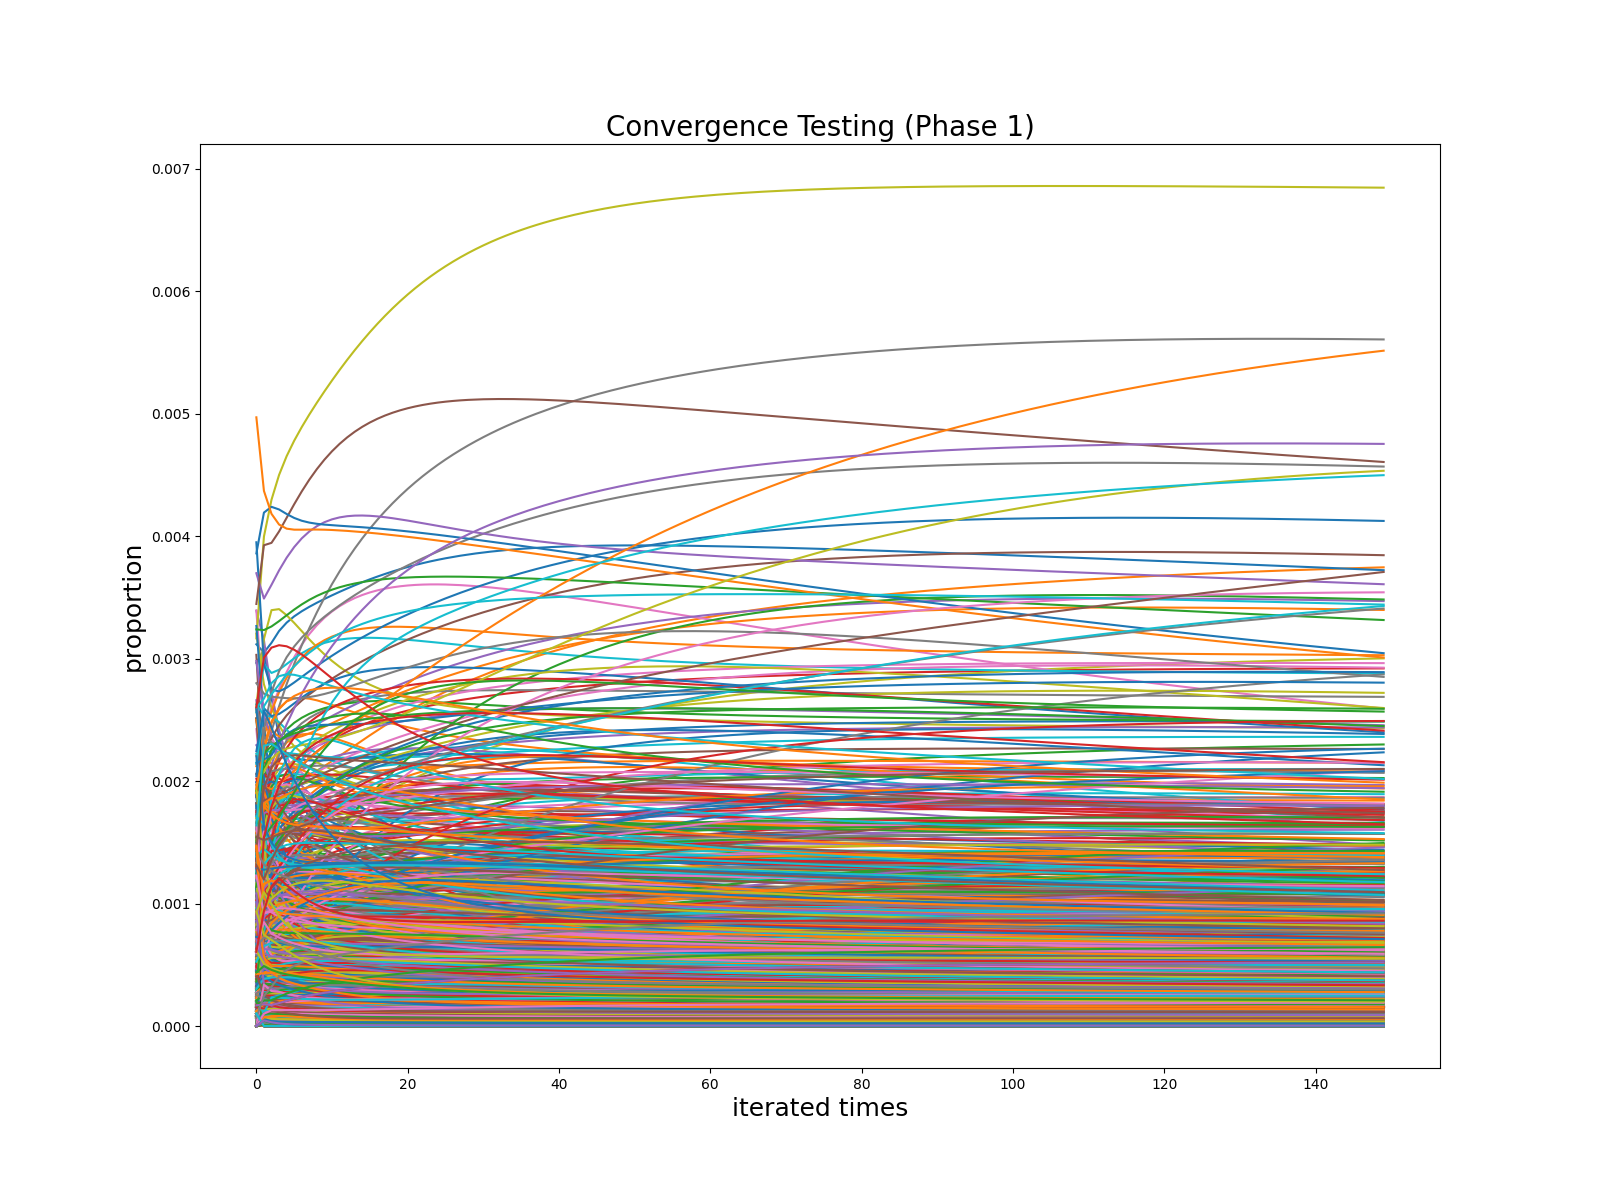
\includegraphics[width=\textwidth]{SD1_dev.png}
    \caption{}
  \end{subfigure}
  \begin{subfigure}[t]{0.8\textwidth}
    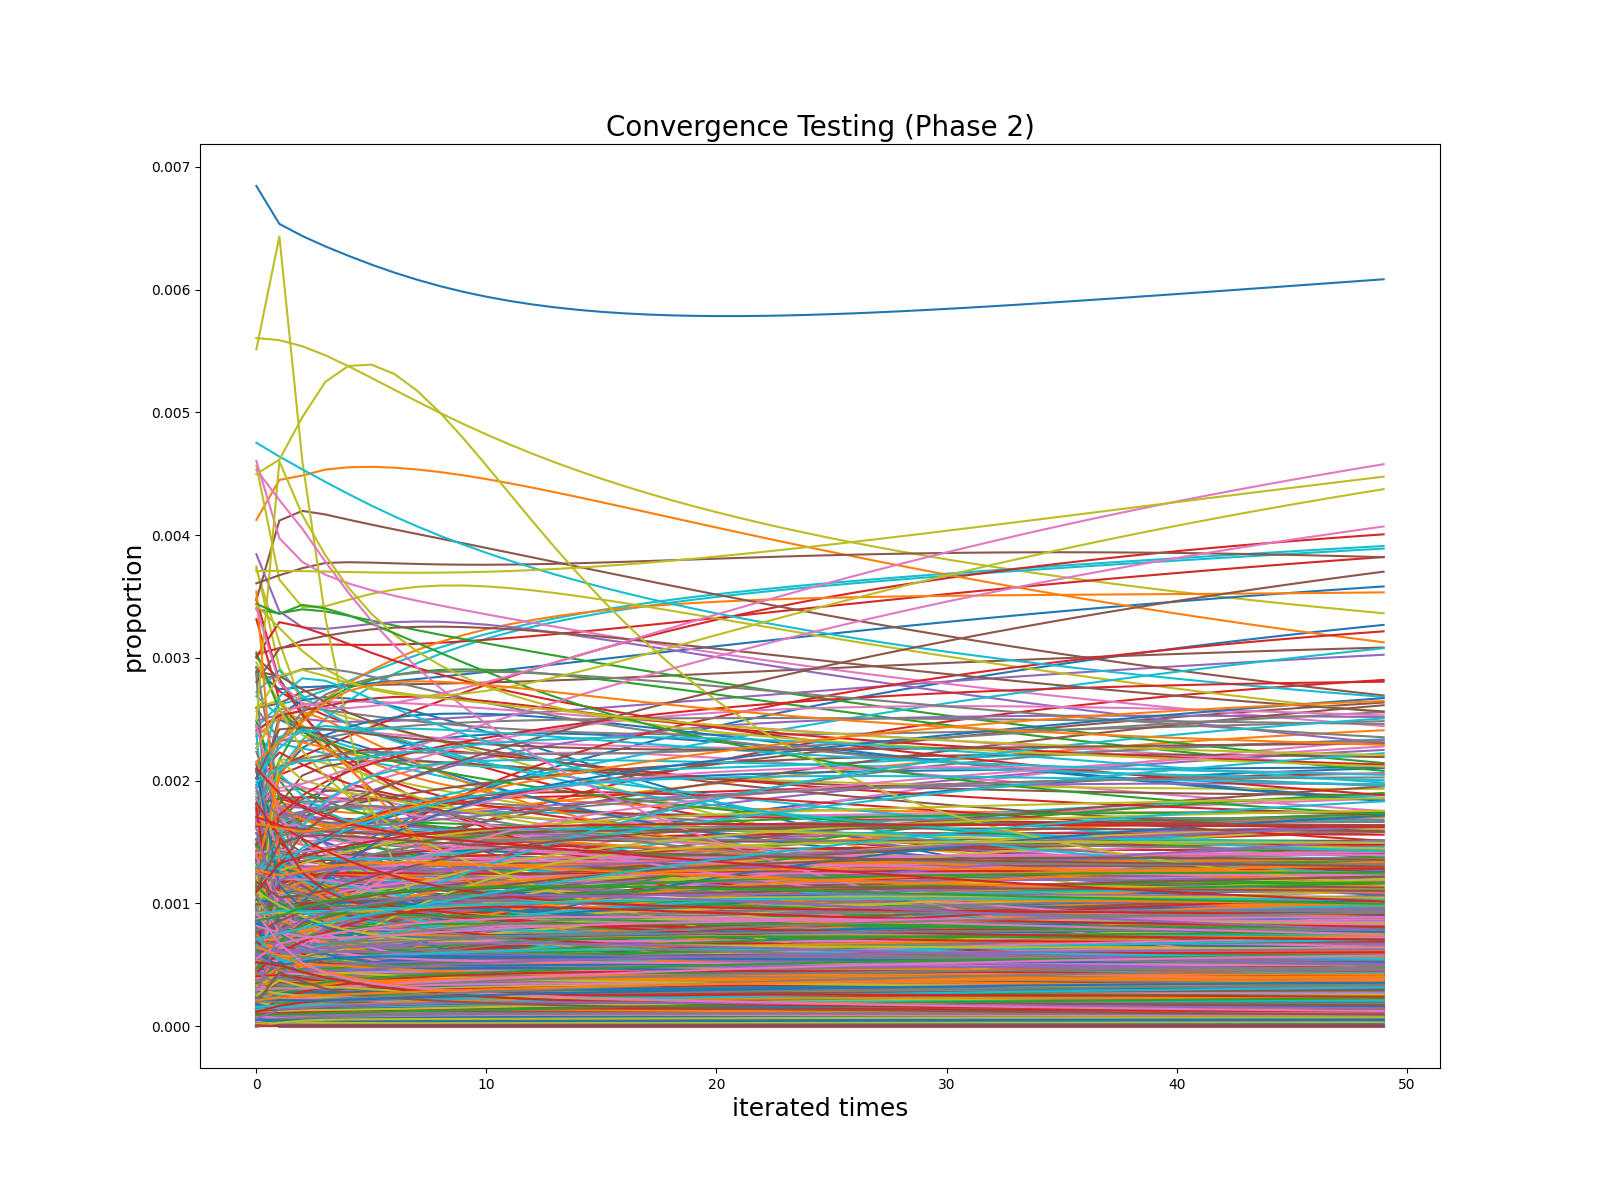
\includegraphics[width=\textwidth]{SD2_dev.png}
    \caption{}
  \end{subfigure}
  \caption{convergence testing in two different phases}
  \label{fig:convergence_test}
\end{figure}

\begin{figure}
  \centering
  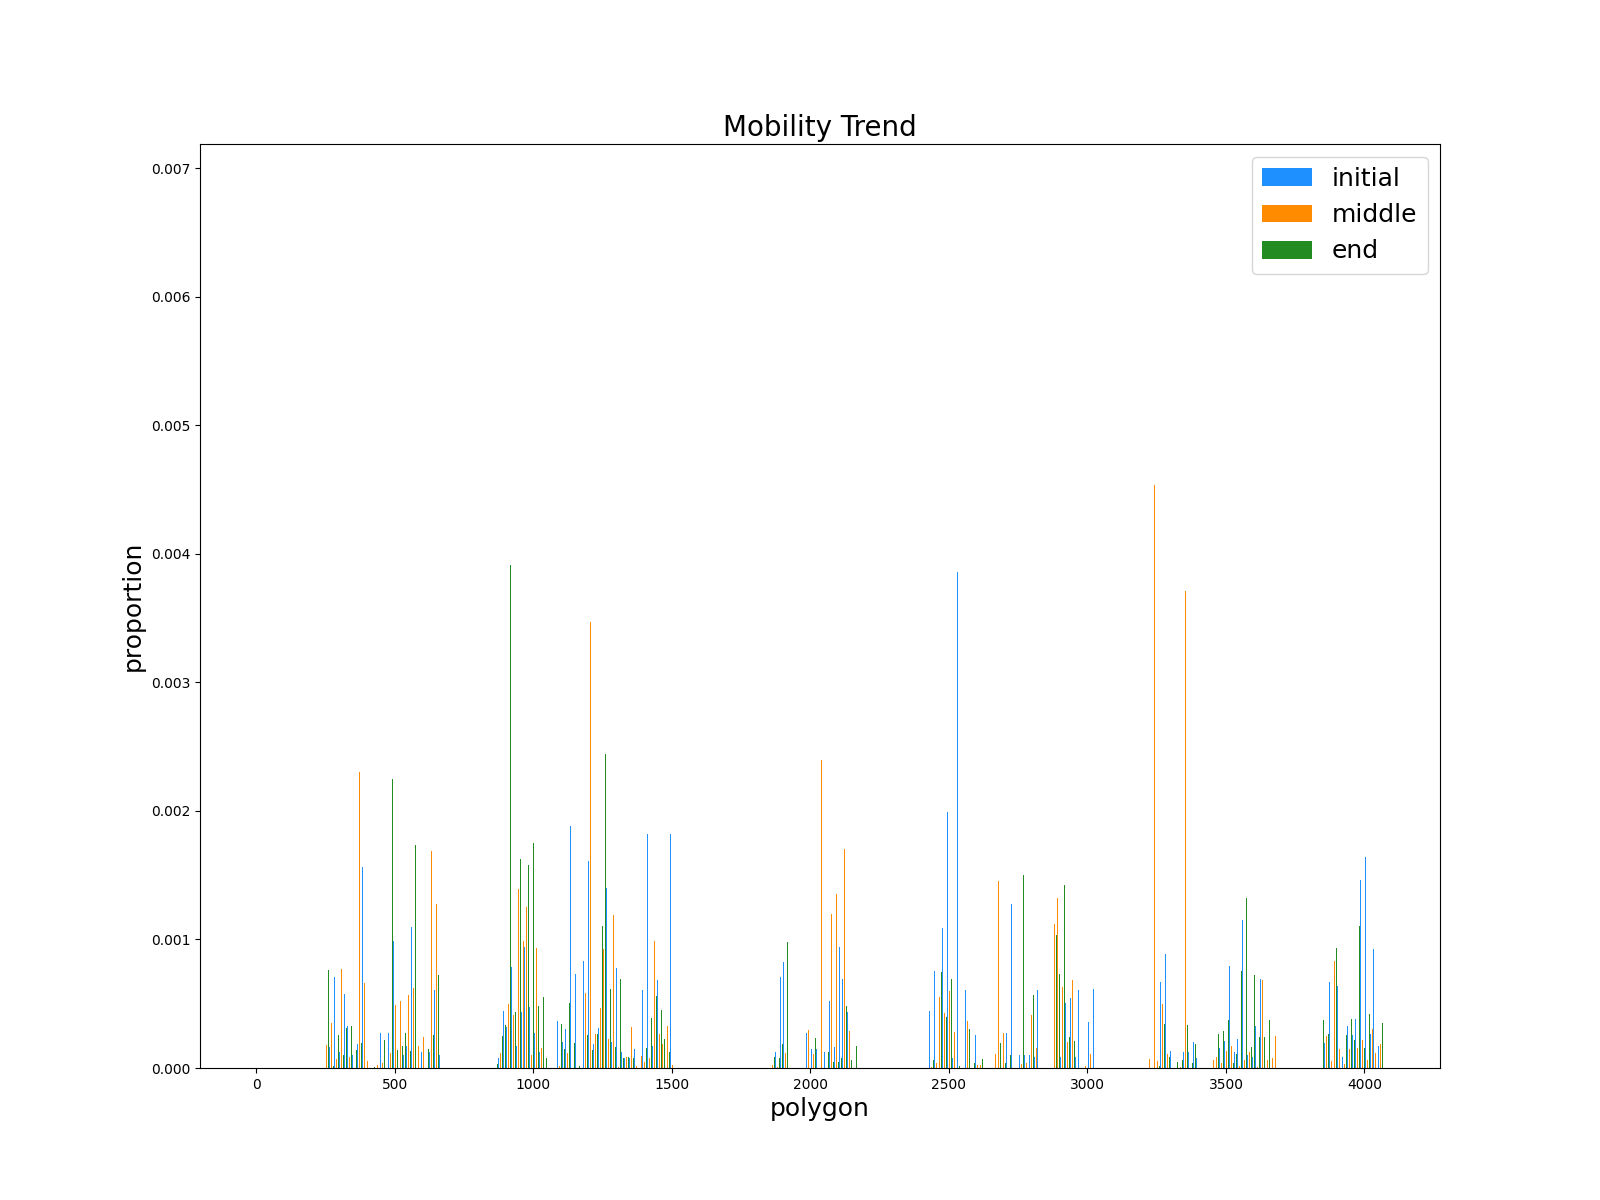
\includegraphics[width=11cm]{SD.png}
  \caption{comparison between intial state and predicted states}
  \label{fig:mob_trend}
\end{figure}


In Figure \ref{fig:mob_trend}, ‘Initial’ represents the initial vector \(\boldsymbol{v}_{0}\); ‘Middle’ is the stationary distribution \(\boldsymbol{\pi}_{1}\) that \(\boldsymbol{v}_{0}\) converges through \(\textbf{P}_{(0)}\) at the end of the first phase, which is 9 am; and ‘End’ is the stationary distribution \(\boldsymbol{\pi}_{2}\) that \(\boldsymbol{\pi}_{1}\) converges through \(\textbf{P}_{(1)}\) at the end of the second phase, which is 10 am. 

To sum up, \(\boldsymbol{v}_{0}\) represents the known population distribution of each area at 8 am; in reality, this can be the last known record used to predict the further. \(\boldsymbol{\pi}_{1}\) and \(\boldsymbol{\pi}_{2}\) are the forecasted distribution at 9 am and 10 am. This whole procedure could be one way of forecasting. We compare each of these distributions at certain time to observe the change in the density in each area. Note that \(\boldsymbol{\pi}_{i+1}\) may not have converged to stationary at the end of the \(i^{th}\) phase if the number of iterations \(n_{i}\) is not large enough.


\subsection{Reformulate Transition Matrix with Simulated Trajectories}
Another way of forecasting is implementing simulation algorithms on empirical models. Given the latest MPN records as the initial state, we can simulate the trajectories of each user as their subsequences based on the empirical time-inhomogeneous Markov models, which can be seen as the simulated MPN records. Algorithm \ref{alg:simulation} is such an algorithm as pseudo code.



\begin{algorithm}
  \caption{Algorithm for simulating trajectories based on empirical time inhomogeneous Markov chain}
  \label{alg:simulation}
  \begin{algorithmic}
    \Procedure{Simulation}{$x^{(t)},y^{(t)}$}
    \Comment{parameters: current coordinate}
    \State \textbf{Transformation} \(pol^{(t)} \gets (x^{(t)},y^{(t)})\) \Comment{pol represents polygon ID}
    \For{\(Matrix_{[i]}, i \in \{1,2,...,N\}\)}
    \For{\(Iterations_{[i]}, i \in \{1,2,...,N\}\)}
    \State \textbf{Draw out} \(Matrix_{[i]}[pol^{(t)}]\) \Comment{row number \(pol^{(t)}\) in this matrix}
    \State \Comment{as \(Vec_{[i],[pol^{(t)}]}\)}
    \State \textbf{Accumulation} \(Vec_{[i],[pol^{(t)}]}\) \Comment{add elements cumulatively}
    \State \Comment{as \(CumVec_{[i],[pol^{(t)}]}\)}
    \State \textbf{RandomGeneration} \(r_{[0,1]}\)
    \State \Comment{random generated number from 0 to 1}
    \State \textbf{Position} \(r_{[0,1]} \in (CumVec_{[i],[pol^{(t)}]}[m],CumVec_{[i],[pol^{(t)}]}[m+1])\)
    \State \Comment{compare r with cumulative vector, find its position}
    \State \(pol^{(t+1)} \gets m\) \Comment{m is the next move}
    \EndFor
    \EndFor
    \EndProcedure
  \end{algorithmic}
\end{algorithm}

\newpage

In this case, before separating the whole matrix time-inhomogeneously, we first consider the entire empirical matrix to be time-homogeneous, which is the matrix with one ring noise (See Figure \ref{fig:tm_1}). We make the simulation entirely based on this time-homogeneous empirical matrix with a sufficient number of times and observe how similar they are between the empirical matrix and the simulated matrix. We expect them to be much alike so that the whole simulation procedure will be more credible. 

By applying Algorithm \ref{alg:simulation} into one ring empirical transition matrix, where, in this case, \(i = 1, iteration = 150\). The comparison result is shown on the next page. (See Figure \ref{fig:sim_tm})

The simulated matrix obtained from counting the transitions in simulated trajectories, is very similar to the empirical matrix, which is the matrix the simulated matrix was based upon. This confirms that our simulation algorithm and transition matrix estimation are being as theoretically expected. 

With the above procedure being confirmed as reliable, we can continue to confirm the theoretical expectation of time-inhomogeneous simulation, and estimation analogous to the above procedure, but with different parameters. One way to make the results meaningful is to generate various simulated transition matrices in each time span that we determined at first, so that we can observe different transition matrices in those time periods we are interested. 

\begin{figure}
  \centering
  \begin{subfigure}[t]{0.6\textwidth}
    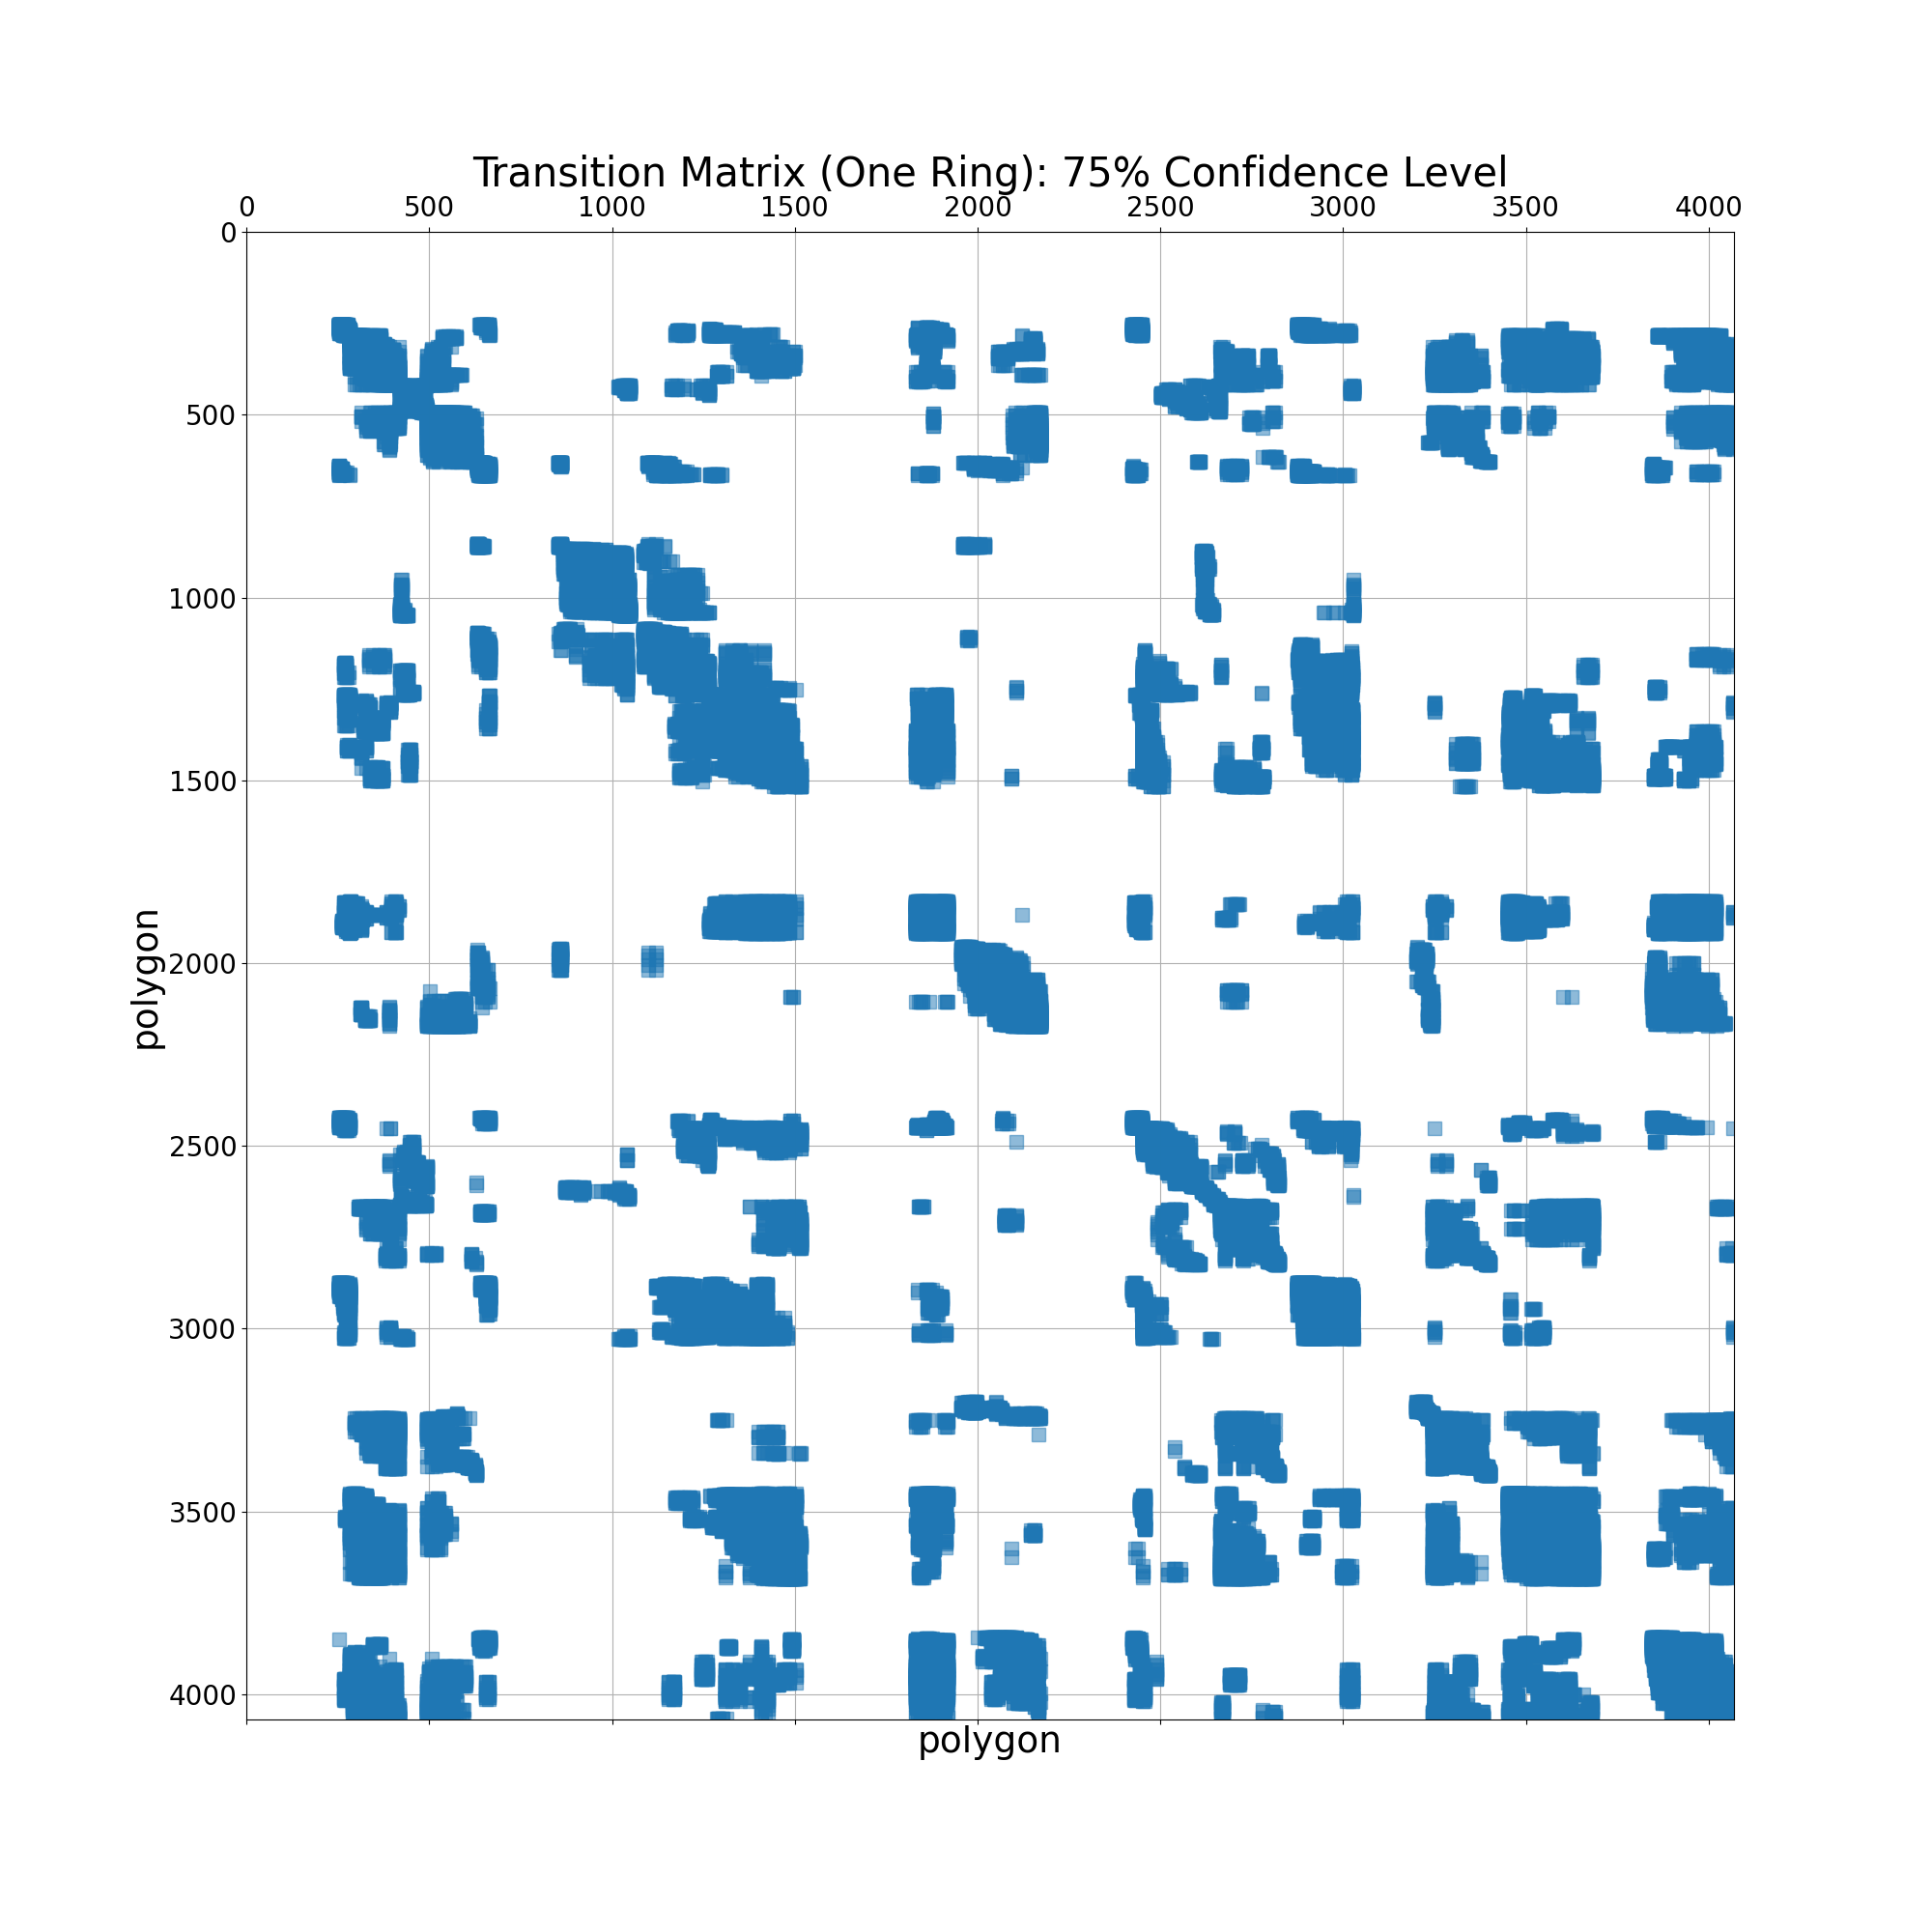
\includegraphics[width=\textwidth]{TM_1.png}
    \caption{}
  \end{subfigure}
  \begin{subfigure}[t]{0.6\textwidth}
    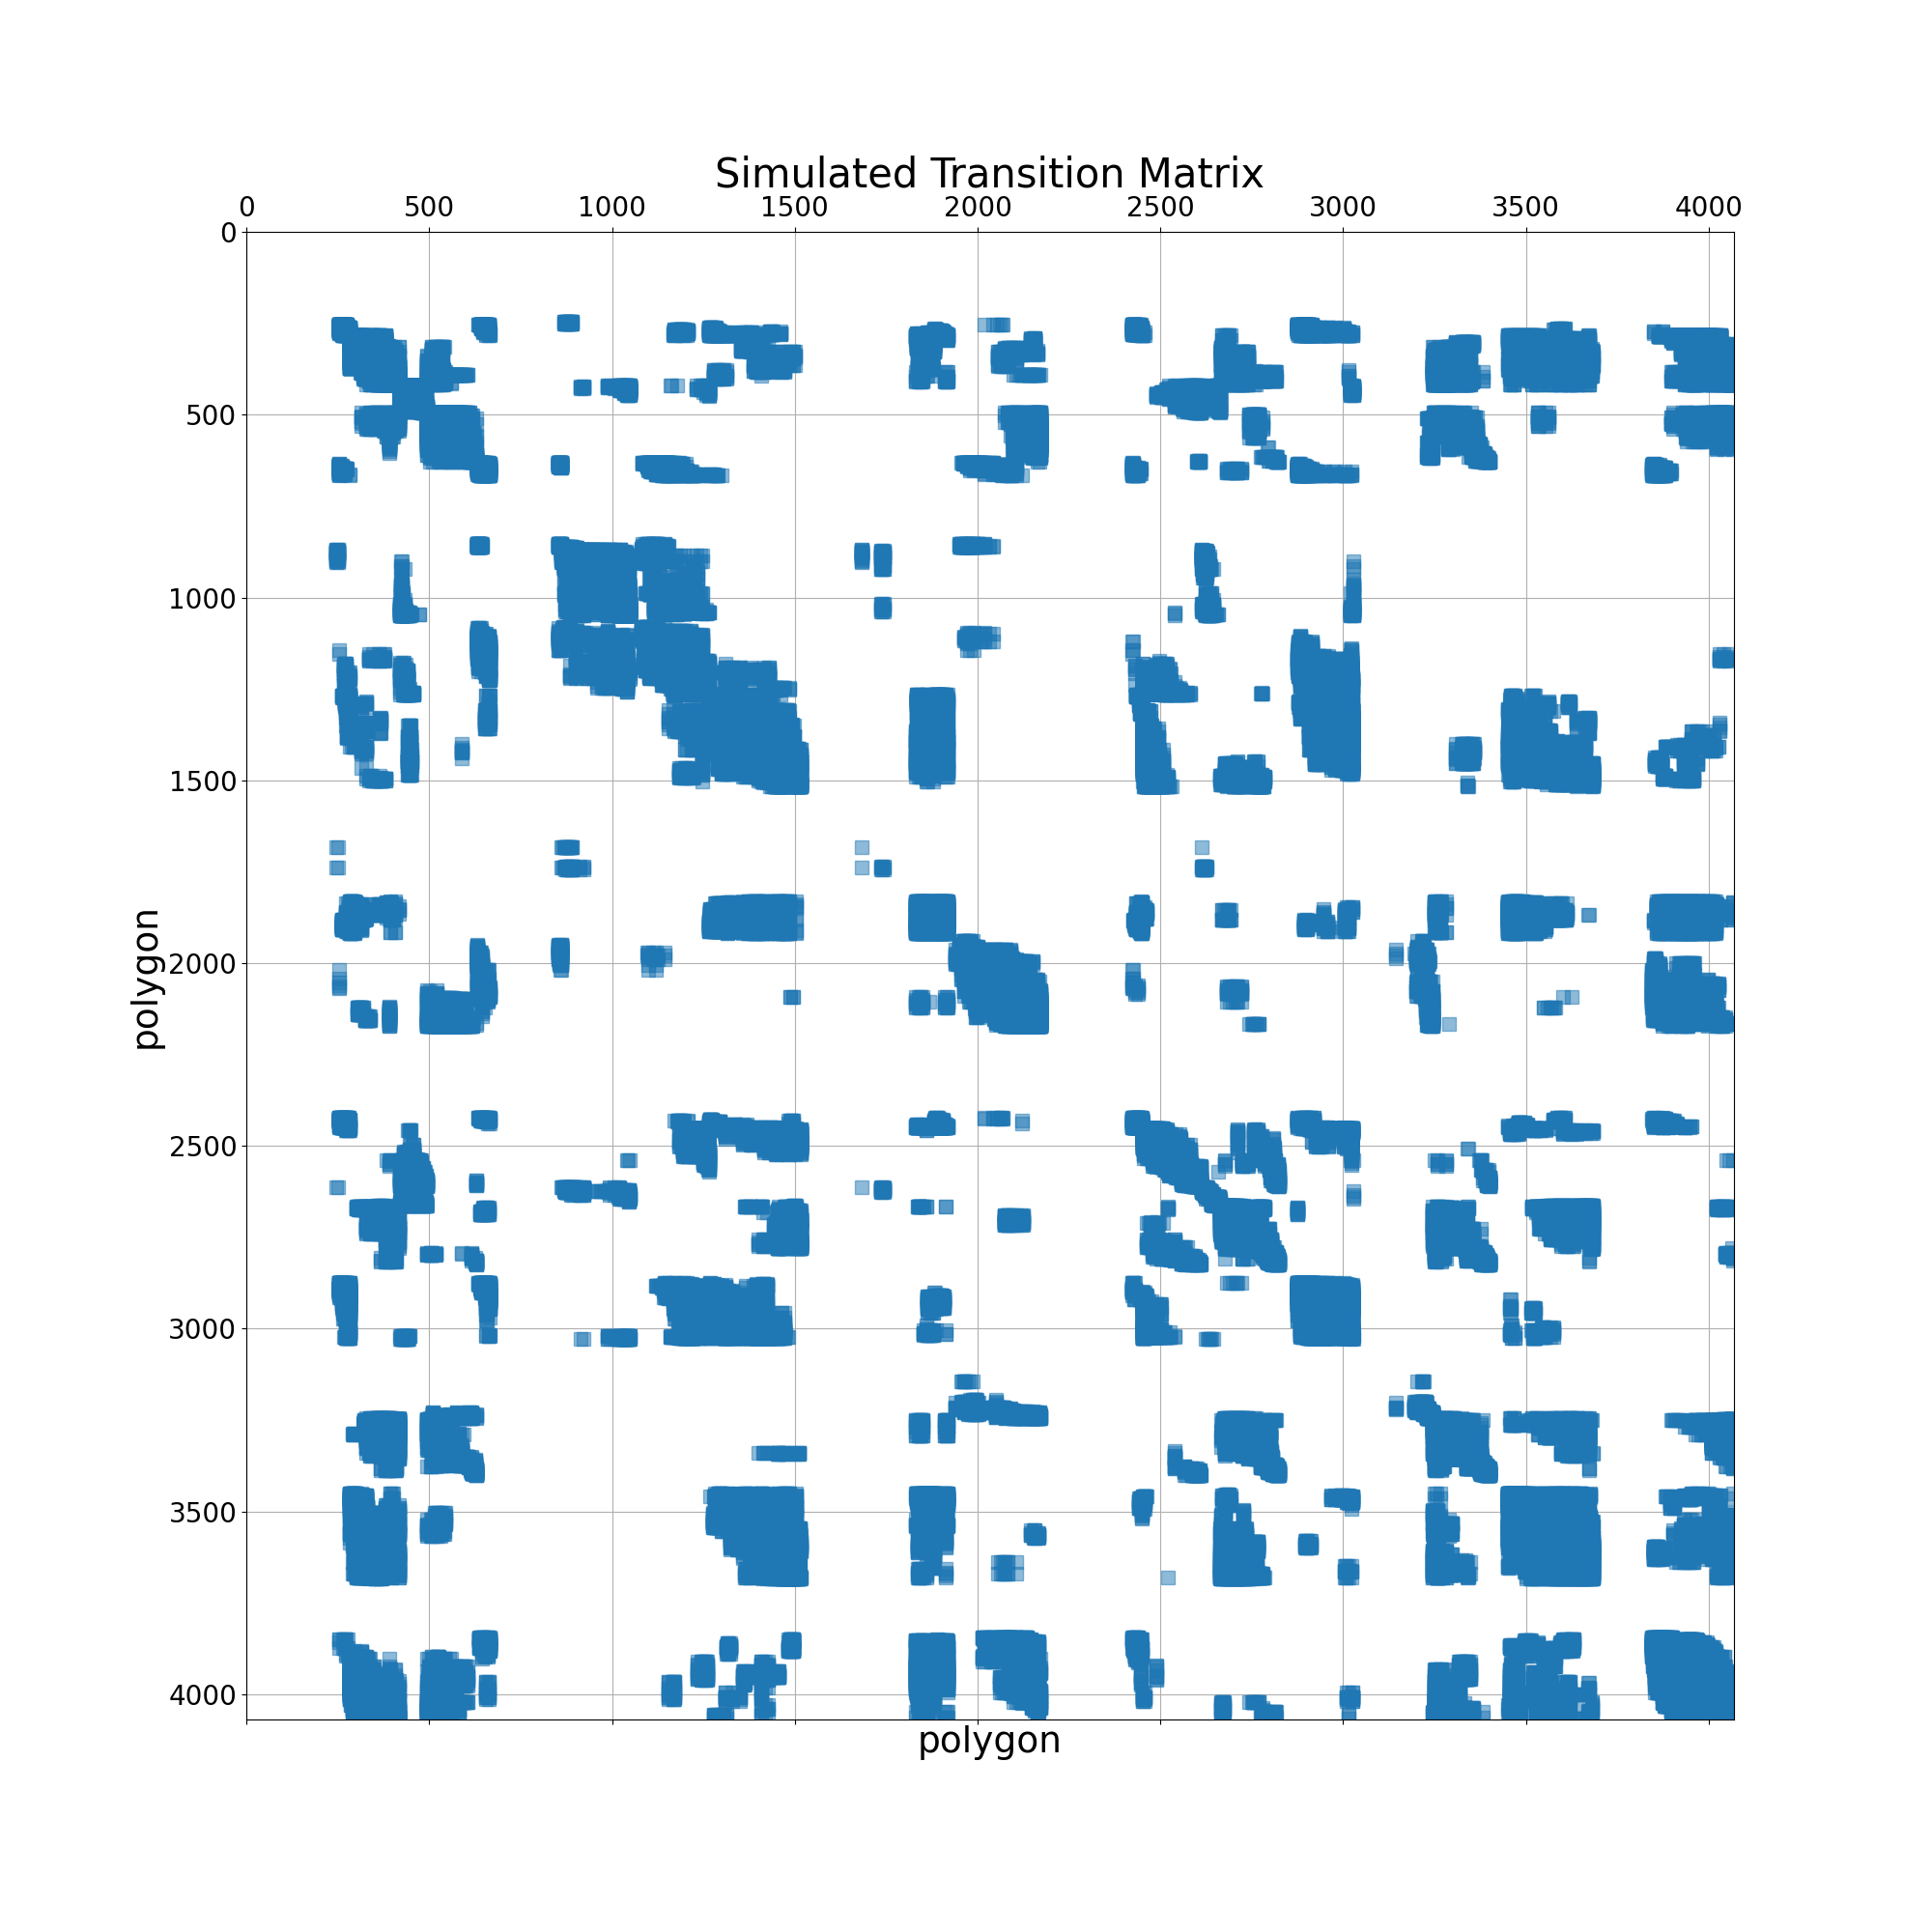
\includegraphics[width=\textwidth]{SIM_TM.png}
    \caption{}
  \end{subfigure}
  \caption{Comparison between Empirical Matrix and Simulated Matrix}
  \label{fig:sim_tm}
\end{figure}




\newpage





%=========================================================%



\section{Scalability Test on Algorithms}
Exploring scalable algorithms for this project along with future related work is also one of our main goals. The above analyses were done on quite a small sample size to focus on the mathematical and statistical description. In this section, we artificially create a large amount of data to test how our algorithms scale with the size of input data. We record how much time will be spent with a different number of compute nodes on the same operation, in order to observe if the operations can be performed on a massive amount of data.

\subsection{Apache Spark and Databricks}
Apache Spark is an open-source unified computing engine and a set of libraries for parallel large-scale data processing on clusters. It can be compiled by multiple widely-used programming languages such as Java, Scala, Python, R, etc. Spark is by far the most actively developed big data framework for developers and data scientists handling big data \cite{spark_guide_2018}. This whole project is designed to be a Geospatial Big Data project to acclimatize to the Spark environment in order to make the most of Spark resources with related studies developed in-depth in the future. Below are some main features of the codes associated with this thesis. The code for this thesis can be found at: \url{https://github.com/lizh7573/distributed_trajectories_mpn}.

\subsubsection{Main Features of the Codes}
\textbf{(1) Pyspark}
This project was done with Spark’s Python API (PySpark). Python is known for its ease of use, along with its comprehensive functionality by providing lots of libraries tailored to data science that can be integrated with Spark. In this project, we imported certain libraries such as NumPy, Pandas, Matplotlib, SciPy, etc., to make this project comparatively easy to be built. However, Spark was originally written in Scala and ran on Java Virtual Machine (JVM), which means our Python codes would have to be translated into codes that could run on the executor JVMs \cite{spark_guide_2018}. This causes Python to be much slower than Scala when it comes to performance. Especially when dealing with big MPN data in the whole range of Sweden or Scandinavia, which may amount to terabytes, performance is an important factor that needs to be considered. We used the following to be able to scale to big data.


\textbf{(2) Spark DataFrame}
The whole Extract-Transform-Load (ETL) procedure was done under PySpark DataFrame. A DataFrame is a distributed collection of data organized into named columns, like a table in a relational database. It preserves the essential features RDD (Resilient Distributed Datasets, architectural foundation of Apache Spark) as immutable, lazy, and parallelized collections. When data were operated under DataFrame with Spark’s built-in libraries, they would be automatically parallelized and distributed across a cluster.


\textbf{(3) Built-in Libraries: Spark SQL, MLlib}
Spark SQL and MLlib libraries are two main libraries we utilized in this project. They are inherent in Spark, thus the so-called built-in libraries. Python libraries we mentioned above are called third-party libraries in this case. Built-in libraries would undoubtedly bring us efficiency and convenience since the whole procedure was framed in its own environment, which is Spark. Spark SQL is built on top of Spark Core that introduced DataFrame as data abstraction, providing Spark with SQL support to manipulate and process DataFrames. As mentioned above, the whole ETL procedure was done in DataFrame in this project, implemented by Spark SQL. MLlib is a distributed machine learning library built on top of Spark Core’s distributed in-memory architecture, primarily used for machine learning and statistical modeling. In this project, we implemented this library mostly for matrix computation (see section \ref{sec:ti_sim}): using sparse vector and sparse matrix brings computational efficiency at scale, especially for data in the form of very large matrices that can be spreaded across multiple machines for operations in distributed linear algebra \cite{matrix_spark_2016}.


\textbf{(4) Broadcast Variables}
When having a large variable to be shared across the nodes or having a smaller table joined by a large table, it would be beneficial to use broadcast operation. Since Spark split up data on different nodes in the cluster, adding ‘broadcast’ operation on such variable and dataframe means sending its entirety to all nodes in the cluster, which would reduce the communication cost and optimize the executions.


\textbf{(5) Repartition DataFrame}
As we mentioned above, data would be natively parallelized by Spark and partitioned into its RDD with a given partition size. The default partition size in Spark is 200, which is not always optimal. Therefore, repartition DataFrame can be used to fine tune Spark as we did in our experiments.

\subsubsection{Introduction to Databricks}
Databricks is a web-based platform for Spark compilation, which provides cluster configurations and IPython-style notebooks. Above is the general view of cluster management in Databricks (See Figure \ref{fig:databricks_cluster}). Basically, Spark Applications consist of a driver and a set of workers (executors). The driver is mainly responsible for responding to user’s program, analyzing, distributing, and scheduling work across the workers, and the workers are responsible for executing the work that the driver has assigned to them \cite{spark_guide_2018}. In Databricks, we can choose different types of drivers and workers. By unclicking the option of Enable Autoscaling, we can also control the number of workers to obtain measures of performance as a function of budget for computing.

\begin{figure}
  \centering
  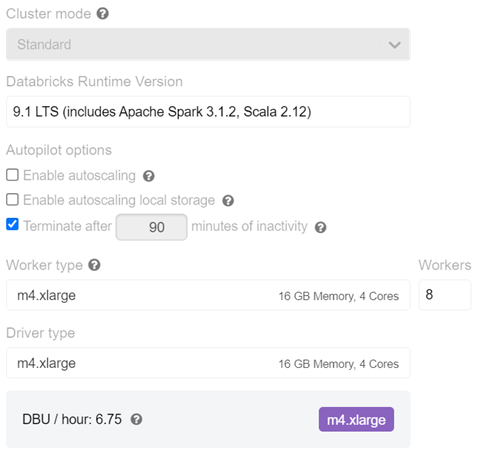
\includegraphics[width=8cm]{Databricks_cluster.jpg}
  \caption{Interface of databricks cluster configuration}
  \label{fig:databricks_cluster}
\end{figure}

For this test, we artificially created different sets of considerable amounts of data, which required somewhat high-performance cluster configuration for both execution and observation purposes. This computing infrastructure was partly supported by databricks University Alliance and AWS credits in the cloud.



\subsection{Testing Results}
We tried to make the artificial data close to the nature of real MPN data so that it could be fitted to our codes and have realistic meaning. We also ensured our codes can scale optimally with Spark DataFrame API and its built-in libraries, use broadcast operations and repartitions. For the test, we chose the construction of the transition matrix as the testing operation (like Figure \ref{fig:tm_1}, which firstly sampled a certain number of users, then simulated some random samples for each user as their trajectories and regarded its order as the timestamp. See Figure \ref{fig:pseudo_traj} for this pseudo-MPN data, where \(simulated\_traj\) represents its location corresponding to the polygon, \(i\) can be seen as the timestamp.

\begin{figure}
  \centering
  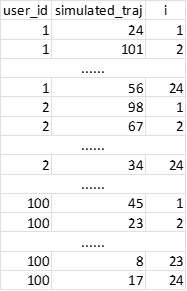
\includegraphics[width=4cm]{pseudo_data.jpg}
  \caption{Pseudo trajectories on 100 random users}
  \label{fig:pseudo_traj}
\end{figure}

Figure \ref{fig:reform_tm} is the result associated with this pseudo data, which does not make any realistic sense, but only highlights its randomness and confirms it is executable. Next, we will make an even bigger size of sample for this test.

\begin{figure}
  \centering
  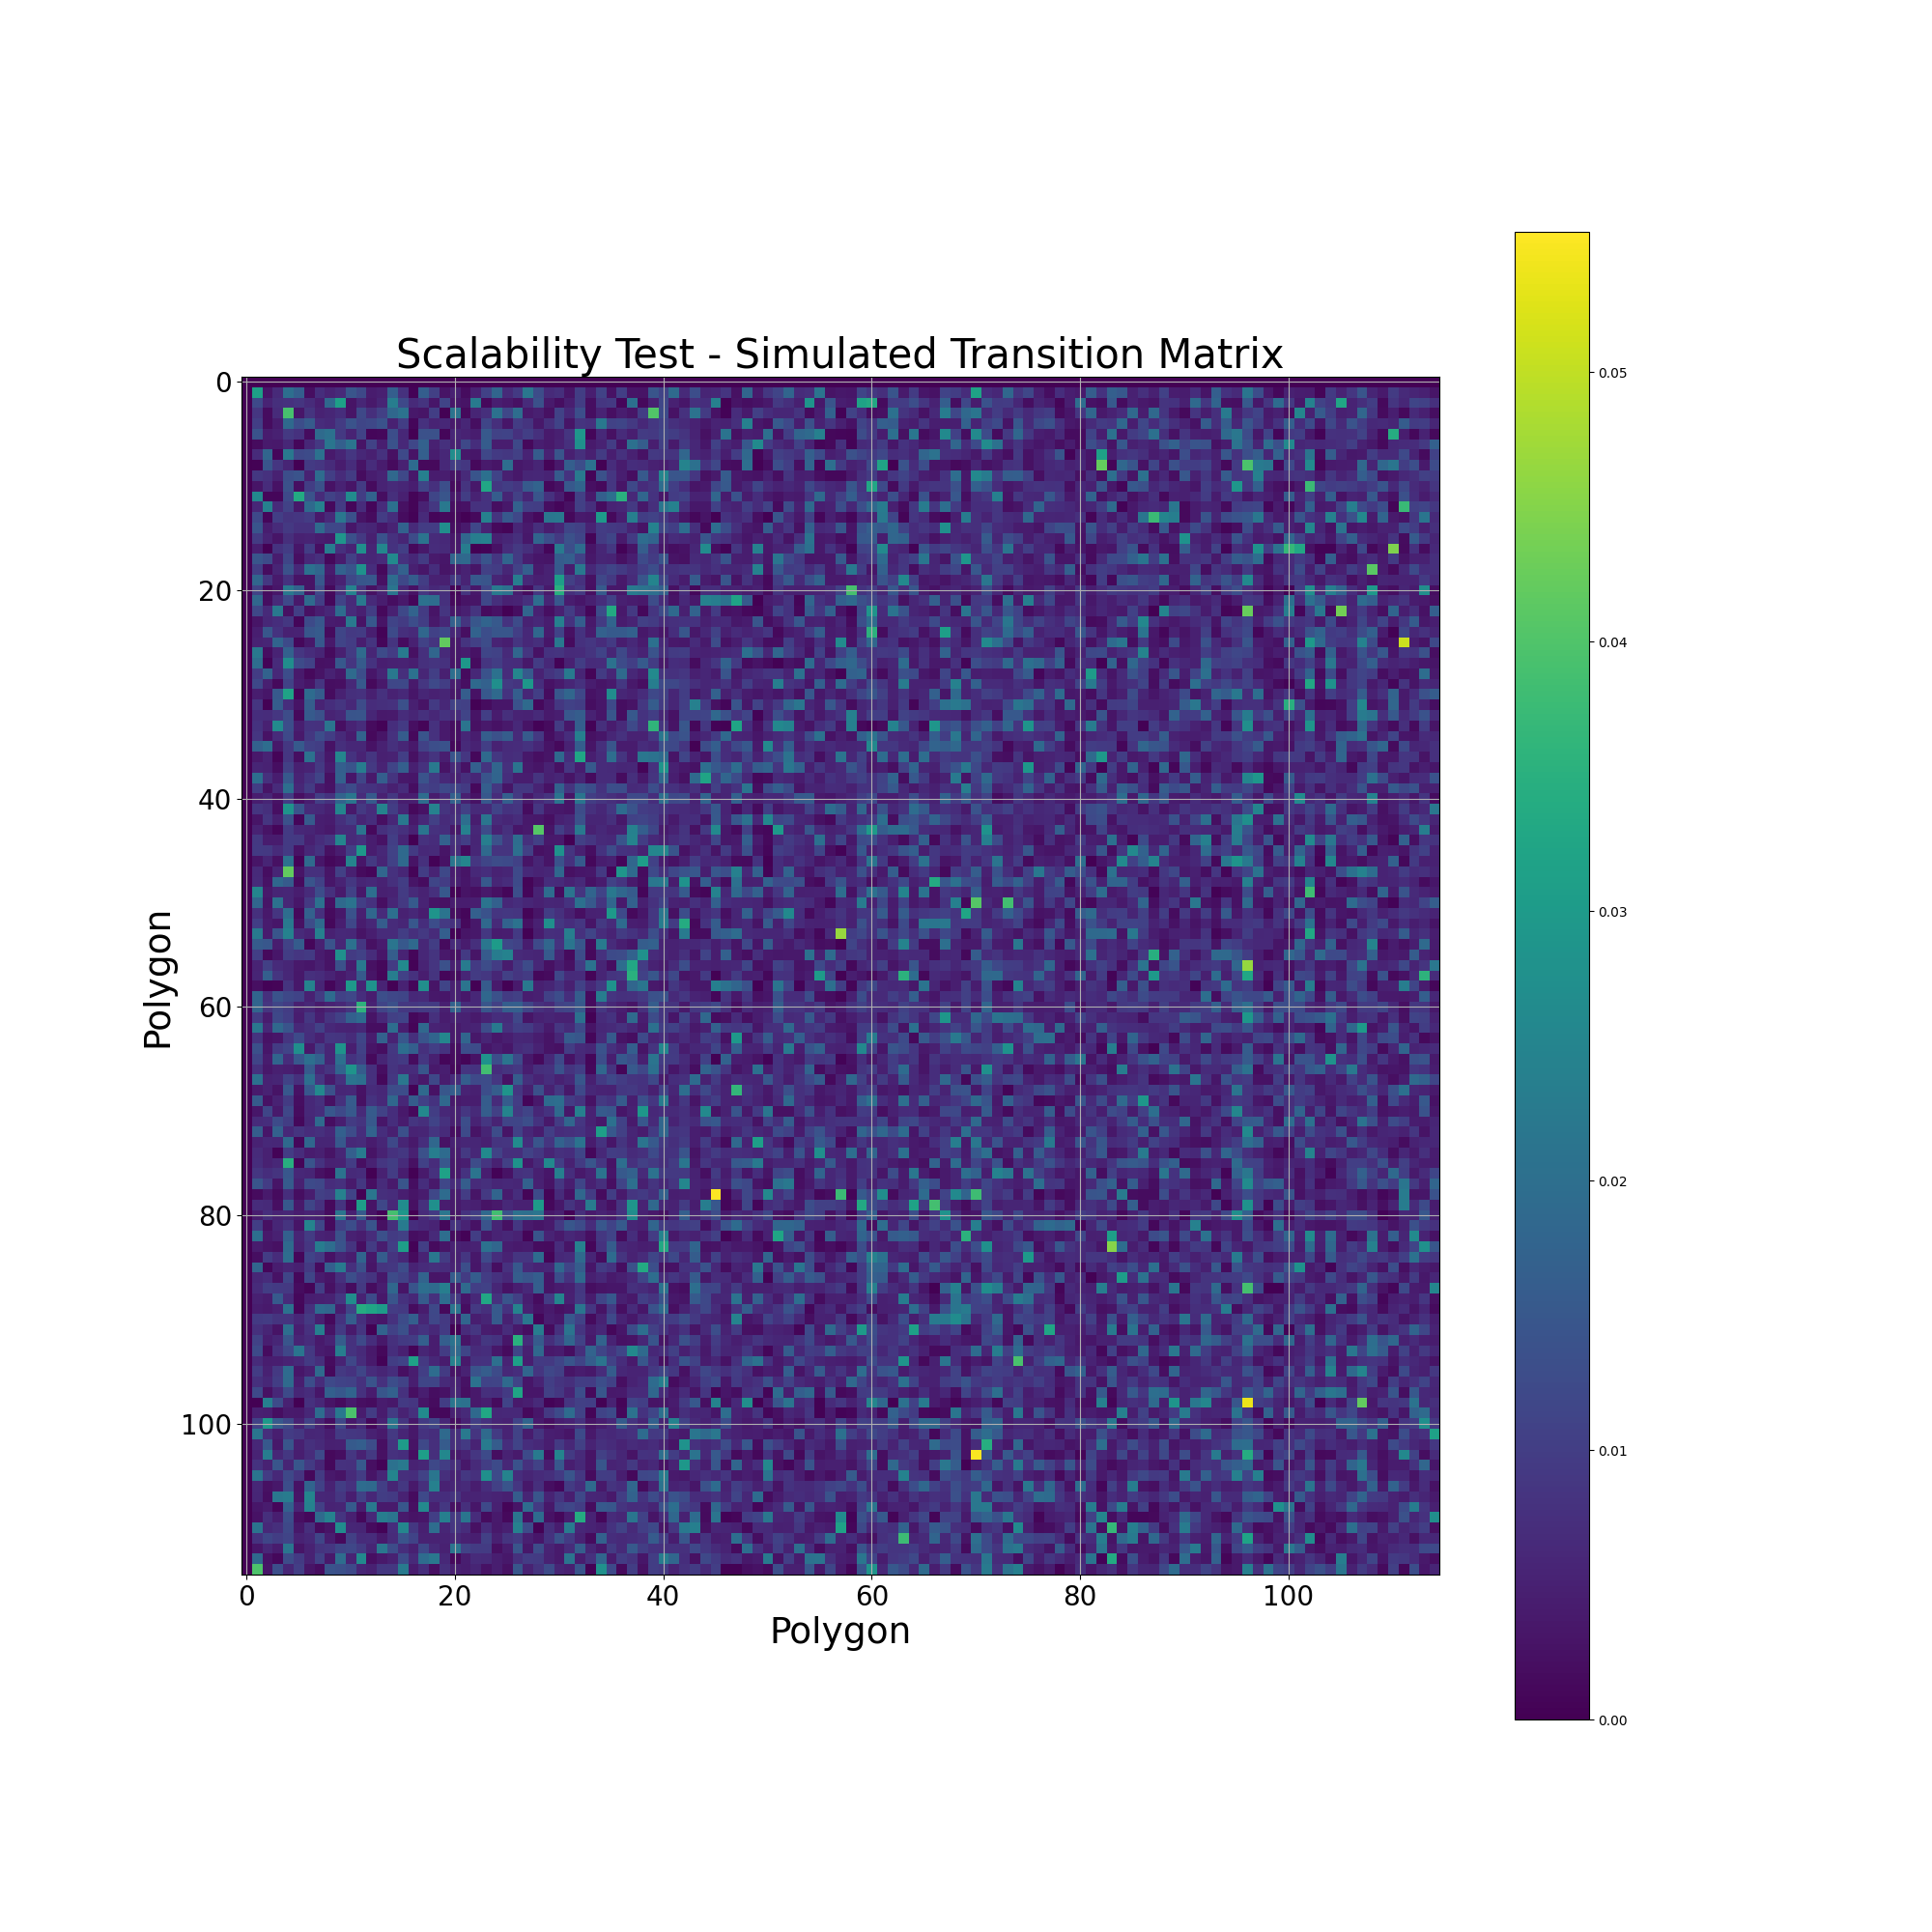
\includegraphics[width=8cm]{TEST_TM.png}
  \caption{Transition matrix based on pseudo trajectories}
  \label{fig:reform_tm}
\end{figure}


Since the real MPN data in this case usually does not have variables other than time and location, we quantified the size of input data by the number of rows instead of the file size, with million as its unit; and the time spent on each task was measured by hour. For each test, the number of users was fixed to 1 million, and only the frequency of their trajectories differs. For example, 1 record per 10 minutes for 1 day amounts to \(6 \times 24 \times 1\) million = 144 million rows, and 1 record per 5 minutes for 5 days is regarded as \(12 \times 24 \times 5 \times 1\) million = 1440 million rows, which should suffice for this test and conformed to form of real MPN data. We controlled the number of workers as the variable. Each worker had 16 GB of RAM and 4 cores. The result is shown in Figure \ref{fig:scalability}.



According to our test result, for fewer workers of the clusters such as 2-workers type and 4-workers type, we stopped increasing size when the time-consumption reached around 5 hours. For 144 million rows of data, with 2 workers it took 4.66 hours, and with 4 workers it took 2.4 hours, reducing half of the time needed by 2 workers; while data was doubled to 288 million rows, 4 workers spent almost the same amount of time as 2 workers did for 144 million rows. The same tendency was between 8-workers type and 16-workers type when data was re-doubled to 576 million. When data increased to 1440 million, that is 1.44 billion rows, the maximum size for this test, 16 workers spent 6.72 hours to finish this task, which was almost the same as we anticipated considering its size and tendency. 


\begin{figure}
  \centering
  \begin{subfigure}[t]{0.8\textwidth}
    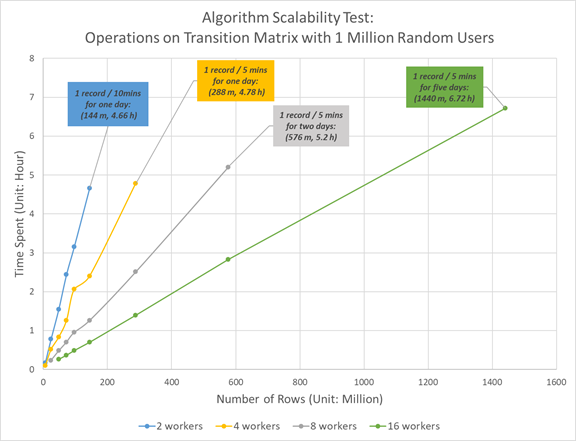
\includegraphics[width=\textwidth]{Scalability_test_1.jpg}
    \caption{}
  \end{subfigure}
  \begin{subfigure}[t]{0.8\textwidth}
    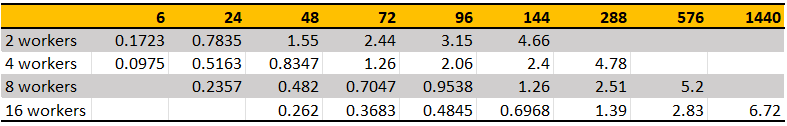
\includegraphics[width=\textwidth]{Scalability_test_2.png}
    \caption{}
  \end{subfigure}
  \caption{Results on scalability test -- operations on transition matrix construction with 1 million random users}
  \label{fig:scalability}
\end{figure}


Considering the fact that this project was done by PySpark, as we mentioned above, the performance can be optimized in Scala. Plus, the pseudo-trajectories data is purely randomized, thus generating the dense matrix instead of the sparse matrix that could have been made by reasonable MPN data. That means the performance could be optimized even more once this whole operation is done by the actual MPN data. However, by observing its tendency as the number of nodes increases, we can come to the conclusion that our algorithm is scalable, which means the capability of this framework can handle a growing amount of work, or possess the potential to be enlarged to accommodate that growth. \newpage


%=========================================================%



\section{Conclusions and Future Work}
In this thesis, we explain the fallacy of the traditional positioning method - Voronoi partition. We reinforce this method from the empirical probabilistic point of view by considering noise on top of it, and use a new concept called distributed trajectories. We present the dynamics of distributed trajectories under the Mobile Phone Network by demonstrating a series of visualizations such as Transition matrix and Origin-Destination matrix. We also implement simulation for application purposes such as forecasting. Last but not least, the codes associated with the thesis are tested as scalable, which is a good start for future work.

This project is more of the starting point of the whole Geospatial Big Data project from the Mathematics Department and the Social Economic Geography Department at Uppsala University, along with the Geography and Human Environment Department at Tel Aviv University. Aside from the performance of the codes we mentioned above, the models and algorithms we implemented are somewhat rudimentary. We also neglected one important factor that should be considered in mobility/trajectory study, which is privacy since the MPN records represent the exposure of people’s trajectories. With regard to this, researchers from Uppsala University have already made some progress \cite{privacy_traj_co-traj_2019}. For future work, we may consider including this element in our research. \newpage

\section*{Acknowledgements}

This work was partly supported by a research grant to Principal Investigator Raazesh Sainudiin titled 
{\em Mobile Phone Data for Society and Privacy for the Individual: From the Conflict to a Synergy in Transport Flows Analysis} 
from Research Center for Cyber Security at Tel Aviv University established by the State of Israel, 
the Prime Minister’s Office and Tel-Aviv University. 

The computing infrastructure was partly supported by databricks University Alliance and AWS credits in the cloud.
\newpage

\bibliographystyle{unsrt}
\bibliography{references.bib}



\end{document}

%%% Local Variables:
%%% mode: latex
%%% TeX-master: t
%%% End:

